\chapter{Analysis}
\label{chap:analysis}

By modeling spatially and spectrally resolved obserations of protoplanetary disks, we can measure their chemical and physical characteristics. To model the system, we generate a synthetic image of what a disk with known physical characteristics (like disk radius, mass, and so on) would look like at a certain distance, inclination, and position angle relative to us. From that synthetic image, we may generate a synthetic set of visibilities, and then compare those visibilities to our observations. By iterating this process, we may generate many models with different parameter combinations and evaluate how well each resulting model disk matches our observations. We use a Markov Chain Monte Carlo technique described in \S\ref{subsection:mcmc} to explore the parameter space and measure the physical properties of the disk.

% It’s not just the aggregation, but rather the iterative process itself that allows us to explore parameter space.  Also, MCMC doesn’t just tell us the best fit values, but, critically, how well we know those values (the uncertainties that we get from the PDF).

In \S\ref{section:gas_model}, we describe the basic equations and computational processes that generate the model disks. In \S\ref{section:param_space}, we describe how, once models are made, we may move through high-dimensional parameter space to identify regions of best-fit. Finally, in \S\ref{section:fitting_procedure}, we present the results of our fitting procedures.


\section{Gas Model}
\label{section:gas_model}

In this work, we use a gas-disk model originally developed by \citep{Rosenfeld2012,Rosenfeld2013} and translated from IDL to Python by \cite{Flaherty2015}. The code assumes that Local Thermal Equilibrium\footnote{This may or may not be a valid assumption in protoplanetary disks, but \cite{Pavlyuchenkov2007} showed that it was appropriate for CO.} (LTE), and hydrostatic equilibrium. The code draws on user-input temperature- and surface-density profiles to calculate a vertical density structure, and calculates the velocity field based on the stellar mass. It then performs radiative transfer on the resulting structure to create a sky-projected image of the model disk, taking into account line thermal and turbulent line broadening. By assuming LTE and hydrostatic equibilibrium, the code is able to to run quickly enough to allow for a Markov Chain Monte Carlo routine to generate models on a reasonable timescale, as described in \S\ref{subsection:mcmc}




\subsection{Establishing Physical Profiles}
\label{subsection:physical_profs}
A circumstellar disk can be characterized by three major profiles: its radial and vertical temperature structures, its radial and vertical density structures, and its velocity field. Generating a model disk is a matter of defining these three functions.


% However, these are complex functions, and the reality that they attempt approximate is not necessarily a well-behaved, simple one; no disk's density actually falls off exponentially, although in some cases it can be well approximated as such (\cite{Hughes2008}, \cite{Williams2011}). Furthermore, even these approximations often cannot be solved analytically, instead relying on numerical integration to be solved, which is a computationally expensive task. Therefore, we choose to make certain simplifying assumptions which, although they come at a cost to realism, enable significantly increased computation speeds.

% Are you specifically talking about the hydrostatic equilibrium condition here?  If so, say it!  I can’t think of anything else that requires numerical integration to solve in the code… unless you’re talking about some sort of arbitrary functional form, but that would not be motivated by theory, and not really by observations either.  There are a lot of good reasons why we assume these functional forms, not just because they’re fast!

% LTE is the only assumption that really increases the computation speed — so if that’s what this paragraph is about you should say it explicitly.  Right now you’re conflating the functional forms of the density/temperature/velocity profiles with the physical assumptions of LTE and hydrostatic equilibrium, so please try to separate those out.  (There is excellent evidence that these disks are well described by a Keplerian velocity profile in hydrostatic equilibrium — that’s basically what Katherine Rosenfeld’s 2013 paper on HD 163296 was about!).  

% Wait, what?  That’s not what LTE means.  Also, you have a 2-D temperature profile, not a 1-D temperature profile!  Do a little more reading about LTE and try again. :-) REWORK


For the disk's temperature profile, we draw on the parametrization of disk temperature structure first laid out by \cite{Dartois2003}, where the disk's temperature is given by,

\begin{align}
  T_{\text{gas}}(r, z) = \begin{cases}
                          T_a + (T_m - T_a) \left[ \cos \frac{\pi z}{2 z_q} \right]^{2\delta} \text{   if } z > z_q \\
                          T_a \text{   if } z \leq z_q(r).
                         \end{cases}
\end{align}
\label{eqn:temp_str}

The atmospheric temperature and mid-plane temperatures are given by $T_a = T_{atm,150} (r/150 \text{AU})^{q}$ and $T_m = T_{mid, 150} (r/150 AU)^{q}$, where $q$ is typically negative and controls the functions' decay. Since $T_m$ is smaller than $T_a$, the second term of the low-scale height temperature function is negative, so the sinusoid effectively implements a decreasingly-negative contribution to the temperature with hight above midplane.  The disk's scale height, controlled by $z_q$ is assumed to be radially increasing, as described by a power law, $z_q(r) = z_{q,150}(r/150 \text{AU})^{1.3}$. $\delta$, a tunable exponent controlling the rate of the disk's vertical temperature decay, is set to 1, though it can take on values between 1-2 (\cite{Dartois2003}).


The disk's velocity field is assumed to be Keplerian with slight corrections for gas pressure support and the addition of a vertical dependence. The assumption of Keplerian veloicites is generally valid in the case that $M_{\text{disk}} \ll M_{\star}$, which continuum observations of the system have shown to be the case for the disks in this system (readers interested in a deeper explanation of the velocity field derivation are referred to \cite{Rosenfeld2013}). With these corrections added, the model disk's velocity field is given by


\begin{align}
  \frac{v_\phi^2}{r} = \frac{GM_\star r}{(r + z)^{3/2}} + \frac{1}{\rho_\text{gas}} \frac{\partial P_\text{gas}}{\partial r};\,\, v_r = v_z = 0.
\end{align}


The final structure we would like to define is the gas density profile. By assuming hydrostatic equilibrium, we may relate the disk's gas density and temperature profiles as

\begin{align}
  -\frac{\partial \ln \rho_\text{gas}}{\partial z} = \frac{\partial \ln T_\text{gas}}{\partial z} + \frac{1}{c_s^2} \left[\frac{G M_{\*} z}{(r^2 + z^2)^{3/2}} \right].
\end{align}

Here $c_s$ is the local sound speed, given by $c_s^2 = \frac{k_B T_\text{gas}}{\mu m_H}$, $T_\text{gas}$ is the temperature profile given above, $m_H$ the mass of hydrogen, and $\mu$ is the mean molecular weight of the gas, set here at 2.37 to reflect the gas's 80\% H$_2$ composition. We may solve this equation by integration, giving us the disk's density profile $\rho(r, z)$.


The model's surface density profile is drawn from \cite{Hartmann1998}, in which they expanded on the work of \cite{LyndenBell1974} to show that the structure of an isolated disk with viscosity given by $\nu \propto R^\gamma$ is well-described by


% Also, isn't this Hughes2008's equation?

\begin{align}
  \Sigma_{\text{gas}}(r) = \frac{M_{\text{gas}} (2 - \gamma)}{2 \pi R_c^2} \left(\frac{r}{R_c} \right)^{-\gamma} \exp \left[-\left(\frac{r}{R_c} \right)^{2-\gamma} \right],
\end{align}


where $R_c$ is the radial extent of the gas disk, $\gamma$ is a power law index, and $M_\text{gas}$ is the total gas mass. This form allows the disk to behave as a power law radially until R$_c$, at which point it turns over into exponential decay. \cite{Hughes2008} showed that exponentially tapering the disk's outer radius, rather than sharply cutting it, provides the best agreement between gas and disk outer radii. We may safely approximate $M_\text{gas} = M_\text{disk}$, since at this early stage in the disk's development, the gas is by far the majority element of the disk's mass total.

% REWORK (on temp freezeout dropoff): Hm, this reminds me that Charlie Qi recently showed that freeze-out is less abrupt than this, so we should probably do something a bit more gradual for freeze-out (I thought Kevin had implemented this, but maybe not in the version of the code that you’re using).  It’s not extremely high-priority, but you should check out Charlie’s (Chunhua’s) papers and make sure you know what I”m talking about and then think about how we could do this better.  


Modifications are made to this density profile in two cases. At sufficiently low temperatures, molecules will condense out of the gas phase. The mid-plane of the disk is sufficiently cold to prompt this behavior. We may simulate this behavior by dropping the gas density by a factor of $10^{-18}$ wherever the temperature falls below some characteristic freeze-out temperature, T$_{FO}$, a temperature which is molecule-specific. Conversely, at the disk's upper surface, photodissociation by stellar and interstellar radiation dominates, so we implement a decrease in density wherever the hydrogen column density at the disk's surface falls below a characteristic value. We use values drawn from \cite{Factor2017} for these parameters, presented in Table \ref{tab:mol_specifics}. The resulting temperature and density structure of a typical proplyd is shown in Fig \ref{fig:temp_dens_str}.


\begin{table}
  \begin{threeparttable}
    \centering
    \caption{Molecule-specific values}
    \label{tab:mol_specifics}
    \renewcommand{\arraystretch}{1.2}
    \begin{tabular}{c  l  c c }
      \toprule \toprule
      \multirow{2}{*}{Parameter} & \multirow{2}{*}{Description}    & \multicolumn{2}{c}{Fixed Value(s)} \\
                                 &                                 & CO, HCO$^+$ & HCN \\
      \midrule %\midrule
      T$_{FO}$            &  Molecular freeze-out temperature      &  19 & 60    \\
      $\sigma_\text{Max}$ & Column density upper limit &  [$1.3 \times 10^{30}] \text{cm}^{-2}$ & $9.5 \times 10^{21} \text{cm}^{-2}$  \\
      \bottomrule
    \end{tabular}
    \begin{tablenotes}\footnotesize
      \item[*] Values drawn from \cite{Factor2017}
    \end{tablenotes}
  \end{threeparttable}
\end{table}



\begin{figure}[htp]
\centering
  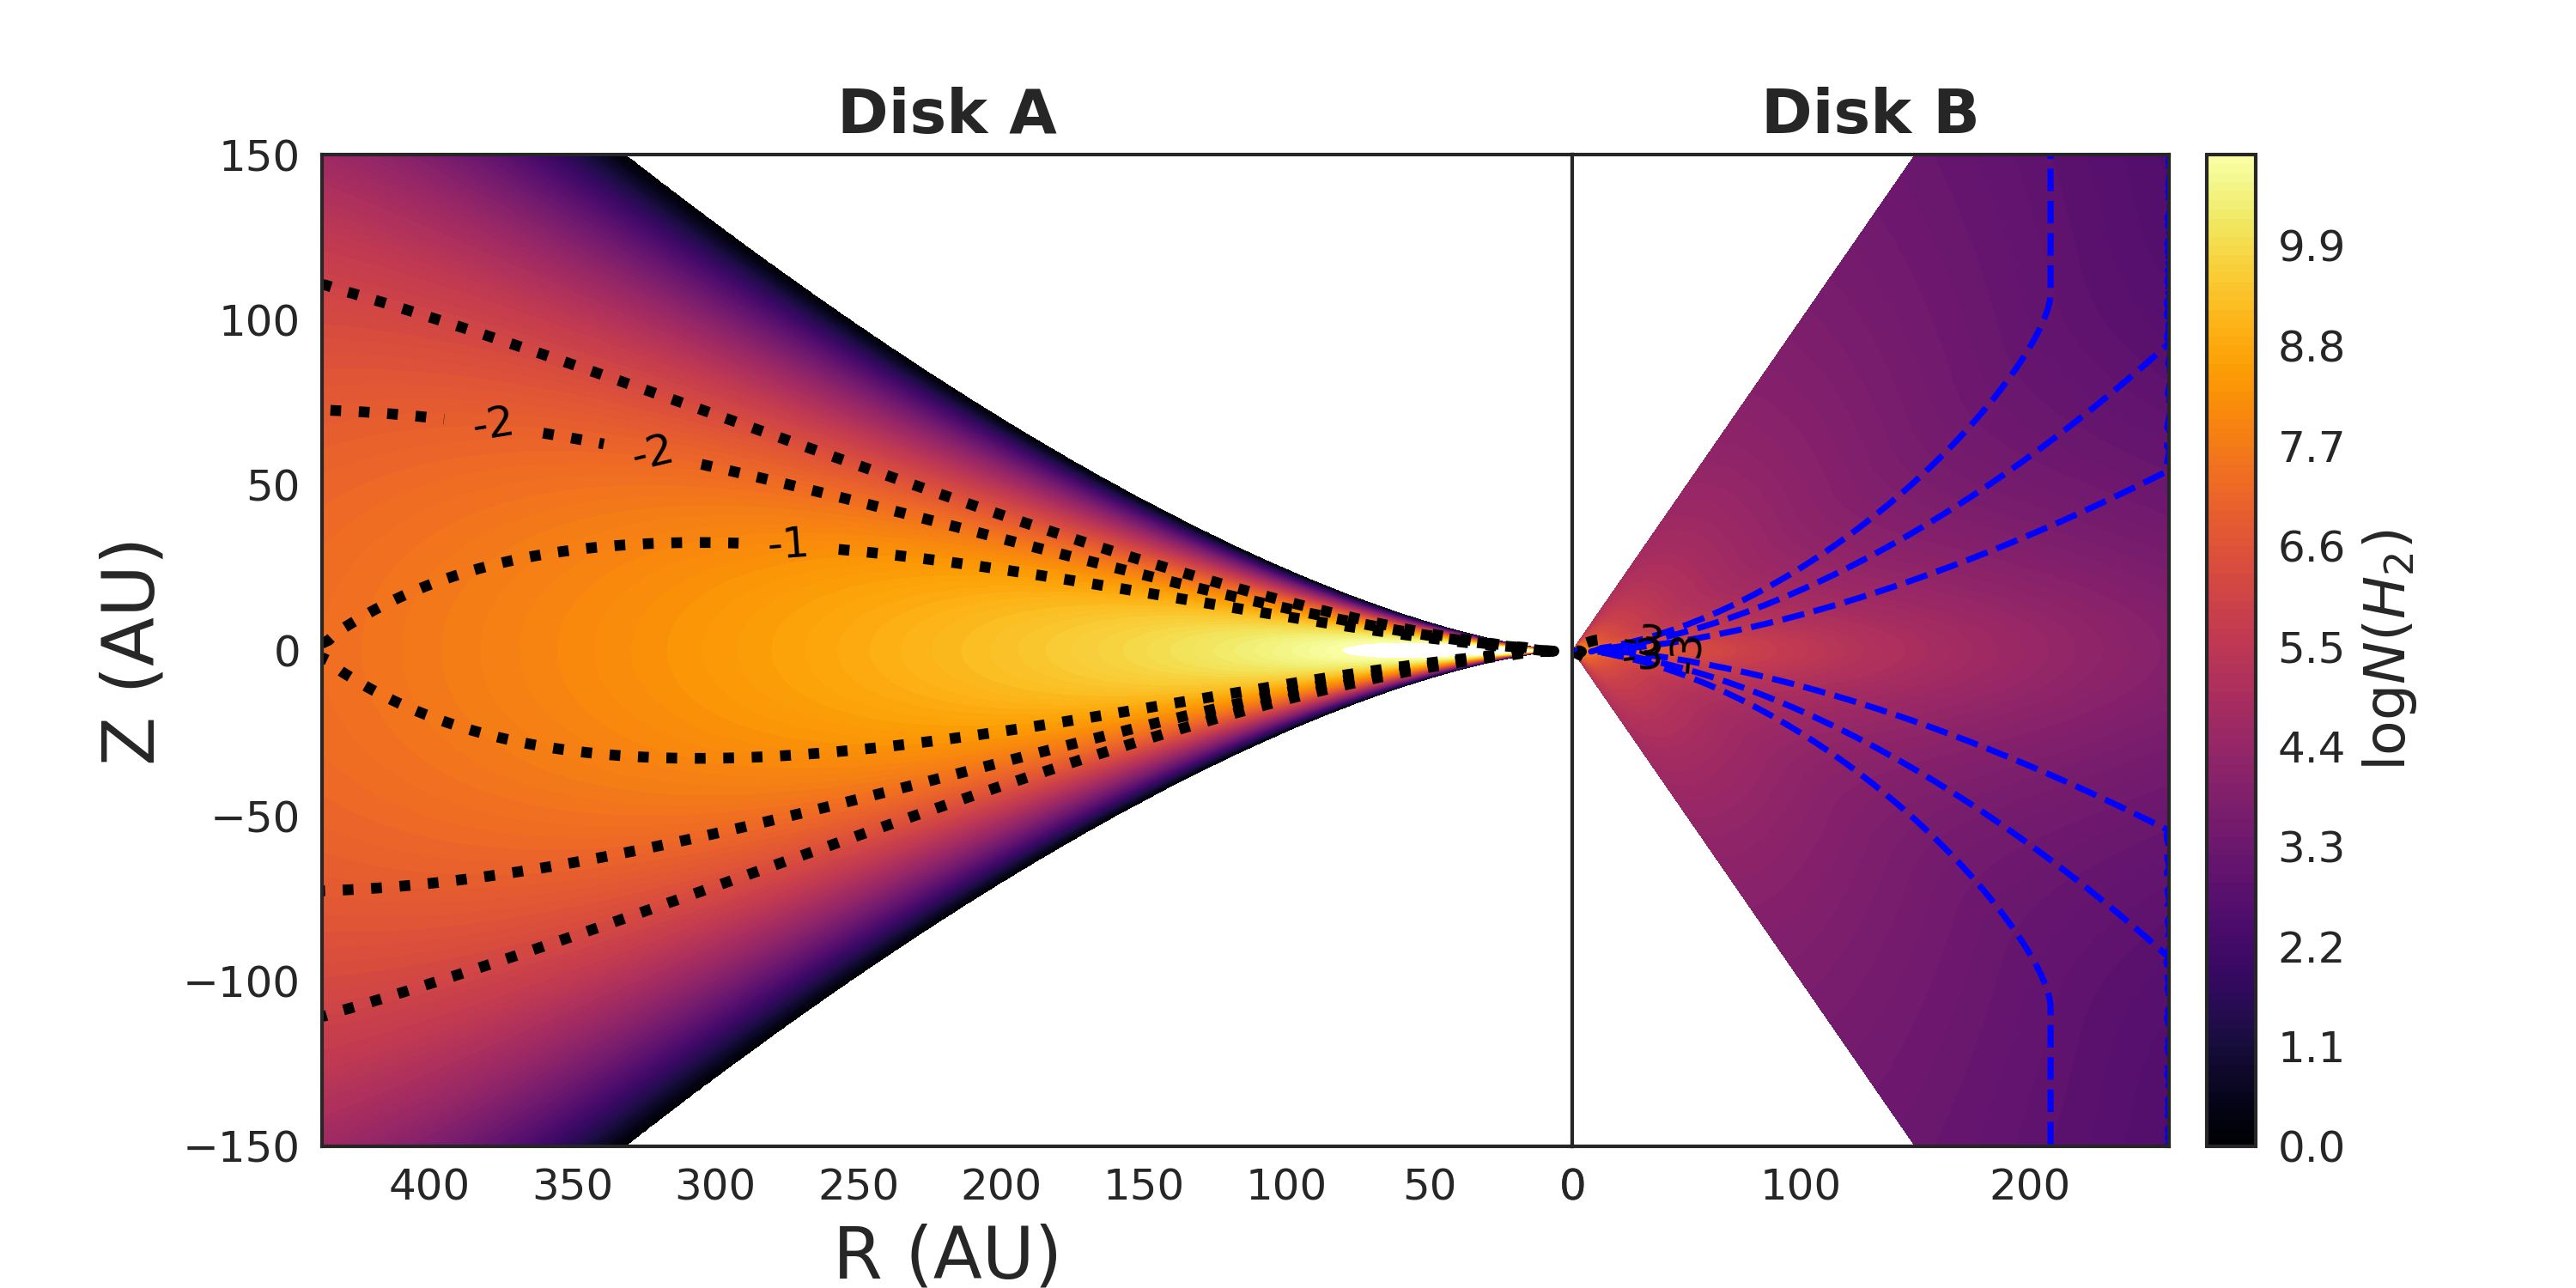
\includegraphics[width=\linewidth]{example-disk-strs.png}
  \captionof{figure}{Radial and vertical temperature structures for disk A \textit{(left)} and disk B \textit{(right)} in CO. We may quickly see that disk A has a larger radial extent and a better defined profile, thanks to its higher signal.}
  \label{fig:temp_dens_str}
\end{figure}
% REWORK: Need a much more informative caption!  Check Sam’s paper for examples if you need them. Also, make the labels bigger on the color bar to the right for readability.  Add units to the label too (both on the color bar and on the contours in the figure).
% I guess go into Kevin's code and chop up? Or just copy/paste it out into analysis or something.





\subsection{Generating a Model Image}

Having now established our model disk's physical structure through temperature, density, and velocity profiles, we may begin generating an image of the disk by calculating flux contributions through the disk. To do so, we calculate the specific intensity by integrating the equation of radiative transfer:

\begin{align}
  I_\nu = \int_0^{\infty} K_\nu(s)\ S_\nu(s)\ e^{-\tau_\nu(s)}\ ds,
\end{align}

where $K_\nu(s)$ is the absorption coefficient, $\tau_\nu(s)$ is the optical depth and is defined as $\tau_\nu(s) = \int_0^s K_\nu(s') ds'$, and $S_\nu(s)$ is the source function. Since disks emit as blackbodies, the Planck function, $B_\nu(T)$, is used as the source function. Line broadening, a function of temperature and disk turbulence, is added, and the resulting flux is Doppler shifted to account for the disk's specified systemic velocity. Finally, the image is scaled, shifted, and rotated to account for the source's distance ($d$), angular offset from the center of the image ($\Delta \alpha$ and $\Delta \delta$), and position angle and inclination (PA and $i$) relative to our viewing direction.
% REWORK: Add an explanation of how I got positional offsets
% REWORK: Baseline cutoff explanation. Does that happen in a different chapter? Maybe should happen here.

Since the model disk is fully defined at every point in both physical and velocity space, we may set the spatial and spectral resolution to ensure that it is sampled well compared to the resolution of the data. We set our spectral resolution to match that of our observation, while we let the spatial resolution be $\sim$ 1/10 the size of the synthesized beam. This resolution is high enough to avoid sampling artifacts when we simulate interferometric observations of the image.

% REWORK: Random thought as I’m reading this: can you please check whether or not Hanning smoothing is implemented in the MIRIAD commands that Kevin’s code uses?  Before uvmodel, there should be a “hanning” command in MIRIAD… let me know.  (If not, we should add it.)

We then use the Miriad task \texttt{uvmodel} to generate visibilities from the model image, sampled in the same $uv$ tracks as our observation. The $\chi^2$ statistic is then used as a goodness-of-fit metric to compare the data and model in the visibility domain. We make this calculation in the visibility domain, rather than the image domain, so that the resulting $\chi^2$ value is not influenced by artifacts generated in the imaging process.


We now have the ability to generate a model disk, first by calculating its physical structures (in radial temperatures, densities, and velocities), then by drawing on radiative transfer to calculate the flux contributions from the disk. That flux is sky-projected to match the observed source's orientation, and the resulting image is then transformed from the image domain to the visibility domain and its fit quality evaluated.



\section{Exploring Parameter Space}
\label{section:param_space}

Now that we have the tools available to generate synthetic images that are tuneable across a large number of parameters, we must decide how best to move through that large parameter space to find a best-fit region. To do so, we use two methods.

\subsection{Grid Search}
\label{subsection:grid_search}
The first, and perhaps most intuitive, way to move through this parameter space is using a simple grid search. A grid search involves manually assembling lists of values to try for each parameter and then generating models and calculating the resulting $\chi^2$ value for every possible combination of parameters in those lists. A best-fit value is recovered by simply finding the point in that $n$-dimensional grid that yielded the best $\chi^2$, and then either calling that position in parameter space a best-fit location or then defining a finer grid around that point and repeating the process until an acceptable resolution has been reached. Benefits of grid search include its relatively straightforward nature (the the consequent simplicity of implementation) and its usefullness as a diagnostic tool, since very specific regions of parameter space may be sampled with the manual entry of positions to test. However, it is a relatively simple method and leaves room for improvement.

Grid search was used to locate the disks in $(\alpha, \dec, v)$ space. All other parameters were fixed at best-guessed values, then grids were run with resolutions sufficiently fine to meet the observations' spatial and spectral resolution. Grids for the disks' systemic velocities were centered at values found in \cite{Williams2014}, while $\Delta \alpha$ and $\Delta \dec$ offsets were first approximated using the MIRIAD task \texttt{uvfit} to fit a Gaussian to each disk. The resulting centroids were used to center the grids for refinement.


\subsection{Markov Chain Monte Carlo}
\label{subsection:mcmc}

Markov Chain Monte Carlo (MCMC) algorithms offer us a way to both sample the probability distribution of a complex parameter space (much like a grid search), but offer an improvement over grid search by yielding the posterior probability distribution of each point, allowing us to characterize the uncertainty associated with each best-fit value with error bars. We use an affine-invariant formulation of the MCMC algorithm described by \cite{Goodman2010} and implemented in the Python package \textittt{emcee} by \cite{ForemanMackey2013}.

MCMC routines sample the probability distribution of a given $n$-dimensional parameter space by deploying an army of "walkers." Each walker begins at some initial position, evaluates the $\chi^2$ value of that point, and then proposes moving to a new position in parameter space according to a Gaussian probability distribution centered at the current point and decaying with distance (so that nearer points are preferentially - but not necessarily - selected). The $\chi^2$ value of this new position - or "step" - is then evaluated, and is either accepted (the walker moves to that position) or rejected (the walker remains where it is and repeats the new-step proposal process) with probability $p = \exp \left[ (\chi_\text{current}^2 - \chi_\text{new}^2)/2 \right]$ (is this only for Metropolis Hastings?). This function indicates that if the proposed step yields a better fit (a lower $\chi^2$ value) than the current position, $p > 1$ and the step is accepted. However, if proposed step results in a worse fit, there is still a non-zero chance that the step is accepted, proportional to how much worse it is. This willingness to accept an increased $\chi^2$ value allows the walker to avoid becoming trapped in local minima. The list of steps taken by each walker and their accompanying $\chi^2$ values are compiled into the "chain" part of Markov Chain Monte Carlo. \cite{Goodman2010} show that a walker's desire to remain in a location is proportional to the local probability density, meaning that we may infer uncertainties in our fits from the density of walker steps taken in a region.

We may introduce boundaries to the parameter space explored by our walkers using "priors." These priors are manually set, and allow us to restrict the walkers' motions into regions that we know a priori to be implausible fits. Justifications for these constraints are either mathematical (e.g. disk should not have a negative radius) or physical (e.g. both disks' radii are clearly far less than 1000 AU). These priors may be either uniform, with hard cuts at their bounds, or Gaussian, with preferential treatment given to walkers closer to the Gaussian centroid (a known value). For this work, we implement a Gaussian prior on each disk's position angle in order to guide the search towards the values reported in \citet{Williams2014} but still allow it the flexibility to self correct if necessary. This prior takes the form of a contribution to the log likelihood function, such that:

\begin{align}
  \text{lnprob} = -\chi/2  -\ln{\frac{1}{\sqrt{2 \pi \sigma_{PA}^2}}} \ex{^{\frac{\text{PA}^2}{2 \sigma^2}}}
\end{align}

for each disk's position angle, where $\sigma_{PA}$ is the position angle uncertainty given by \citet{Williams2014}.



We may visualize the results of the walkers' journeys using corner plots. Corner plots allow high-dimensional space to be visualized in two dimensions by taking slices across each pair of axes and showing the density of samples drawn in that slice. In each of these slices, a perfectly certain fit would appear as a very tight, point-like Gaussian - the sample density around the best fit would be extremely high and low everywhere else, as the walkers quickly converged and remained on that best fit point - while conversely, higher uncertainties are shown by a wide spread of samples around the central point. Degeneracies between parameters can be seen as streaks in these corner plots, showing a correlation. Corner plots for Disk A and B in an HCO$^+$ fit are shown in Figs \ref{fig:corner_a} and \ref{fig:corner_b}, respectively.


\begin{figure}[htp]
  % Maximum length
  % \subcaptionbox{1a\label{fig1:a}}{\includegraphics[width=1.6in]{example-image-a}}\hfill%
  % \subcaptionbox{1b\label{fig1:b}}{\includegraphics[width=1.6in]{example-image-a}}%
  % \bigskip
  % Equal length
  \hspace*{\fill}%
  \subcaptionbox{Disk A fits \label{fig:corner_a}}{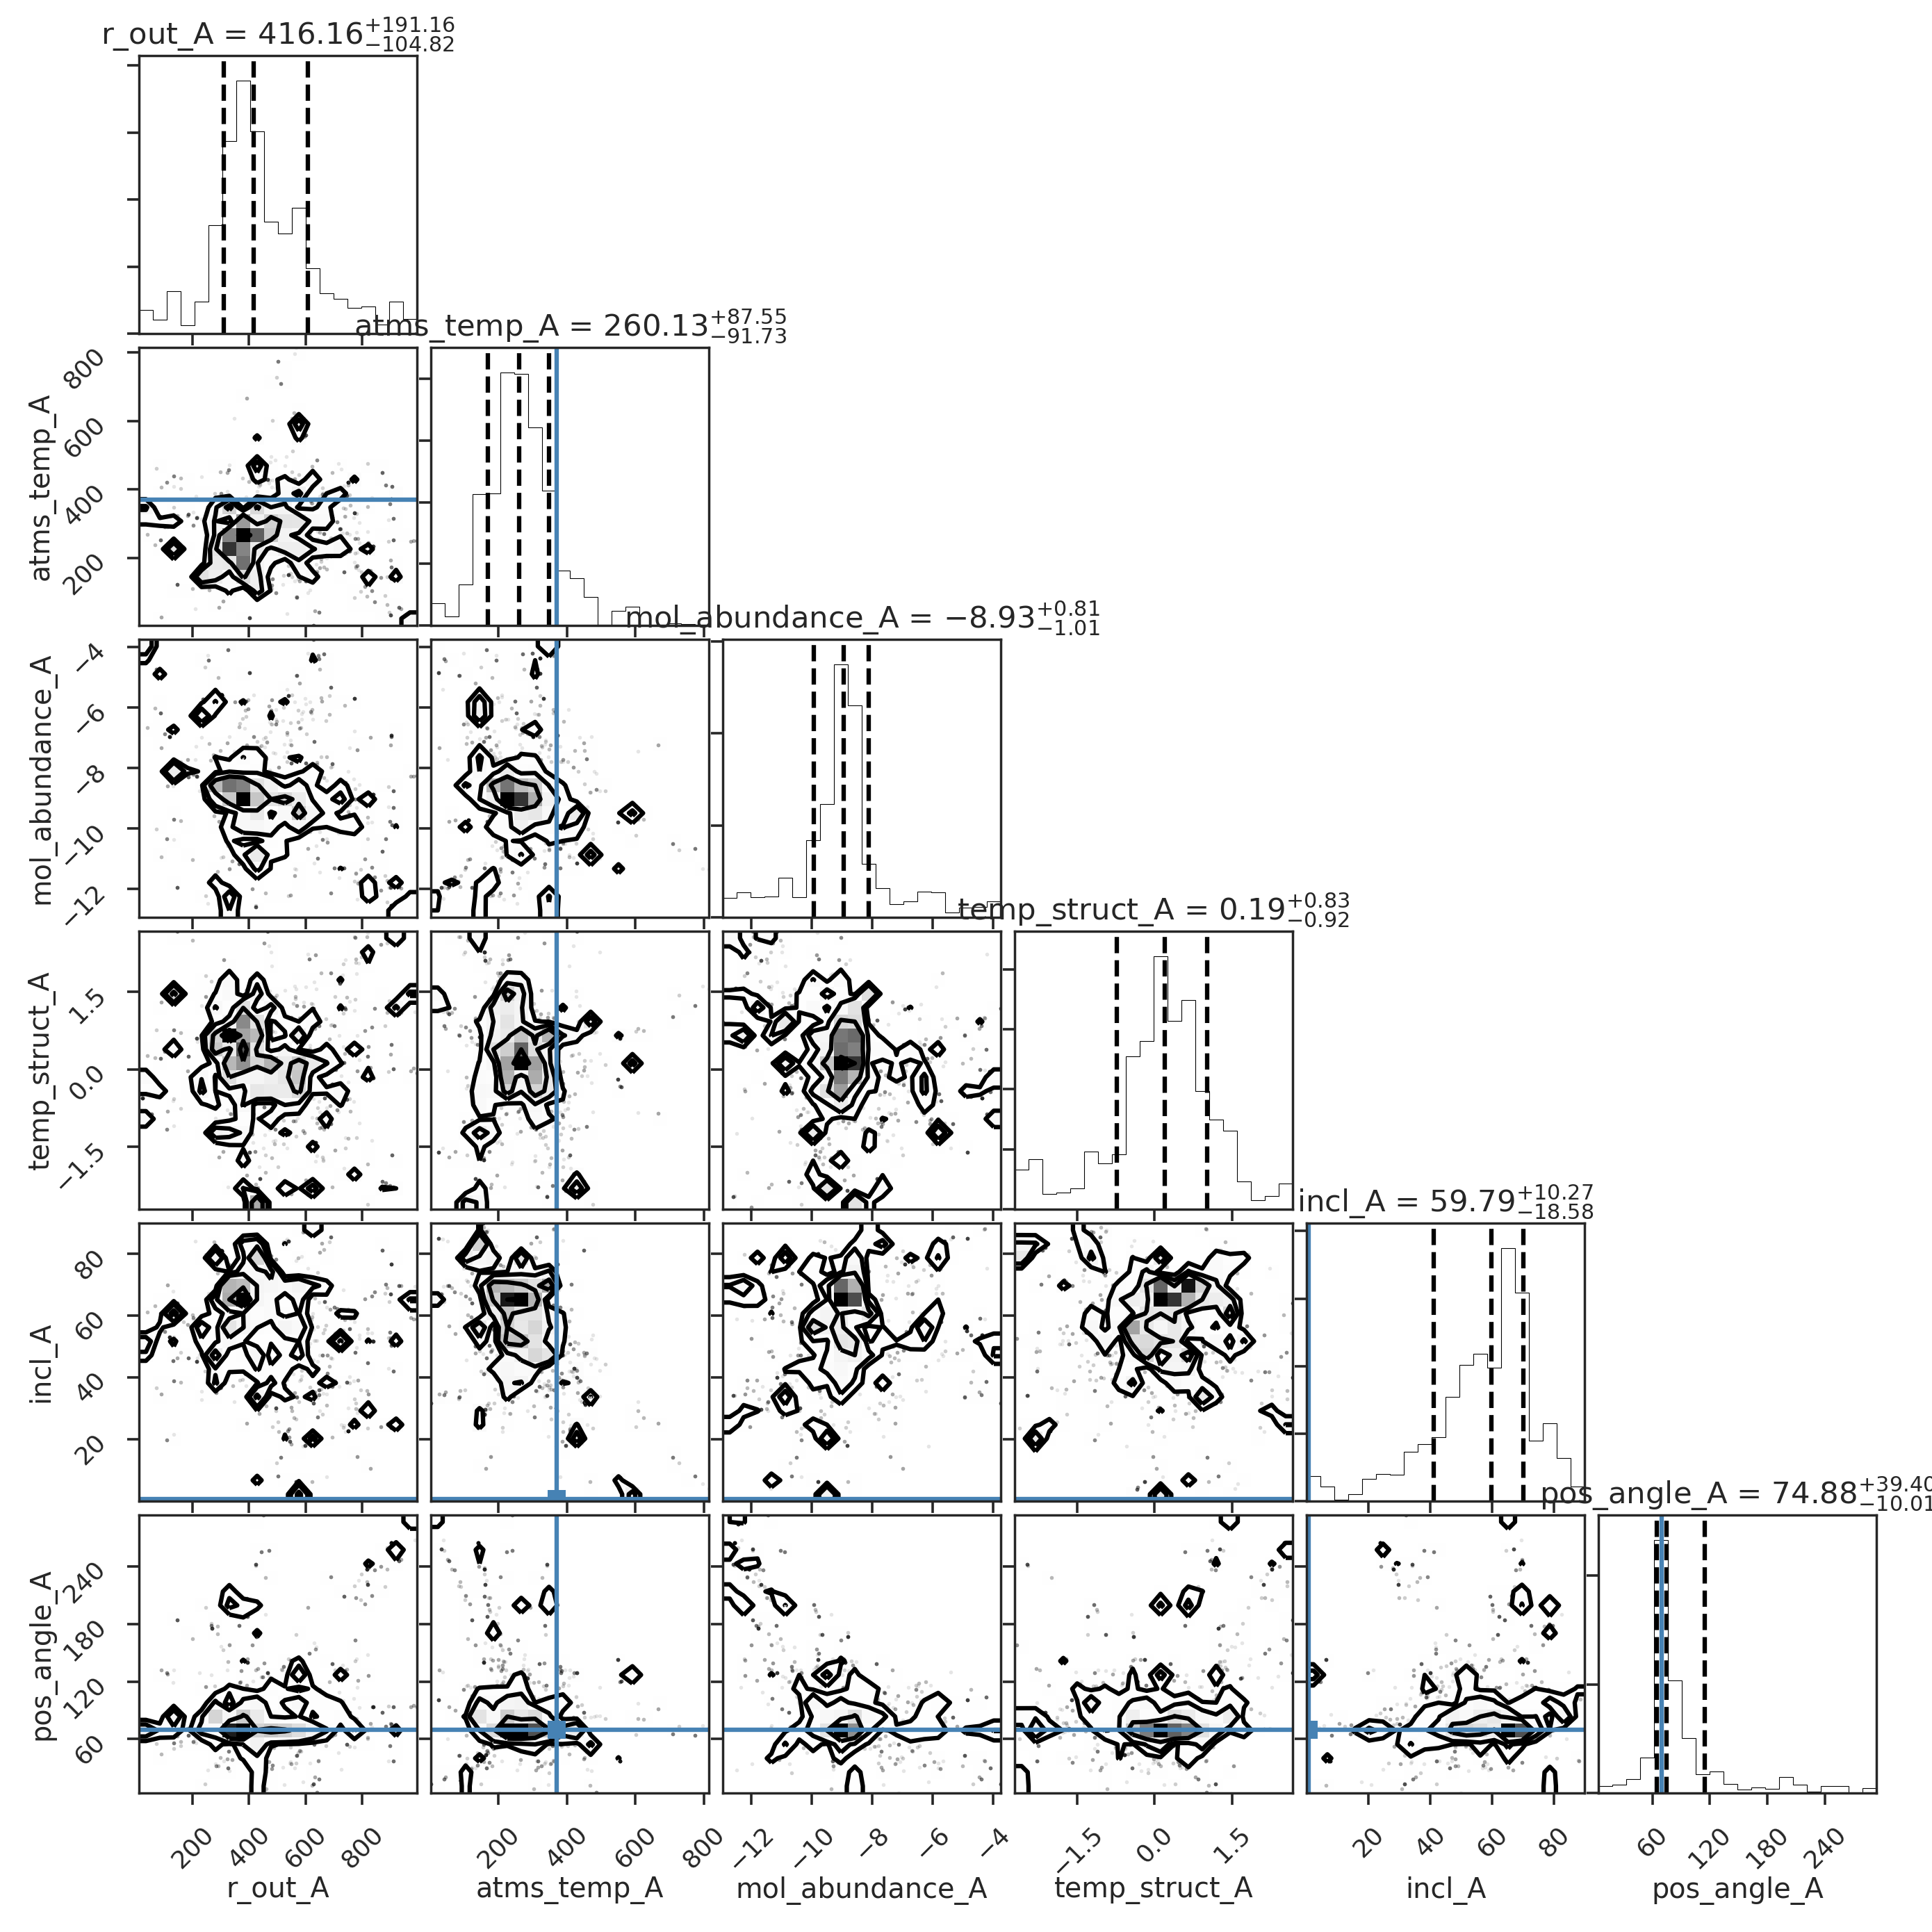
\includegraphics[width=0.49\linewidth]{cornerplot-diskA.png}}\hfill%
  \subcaptionbox{Disk B fits \label{fig:corner_b}}{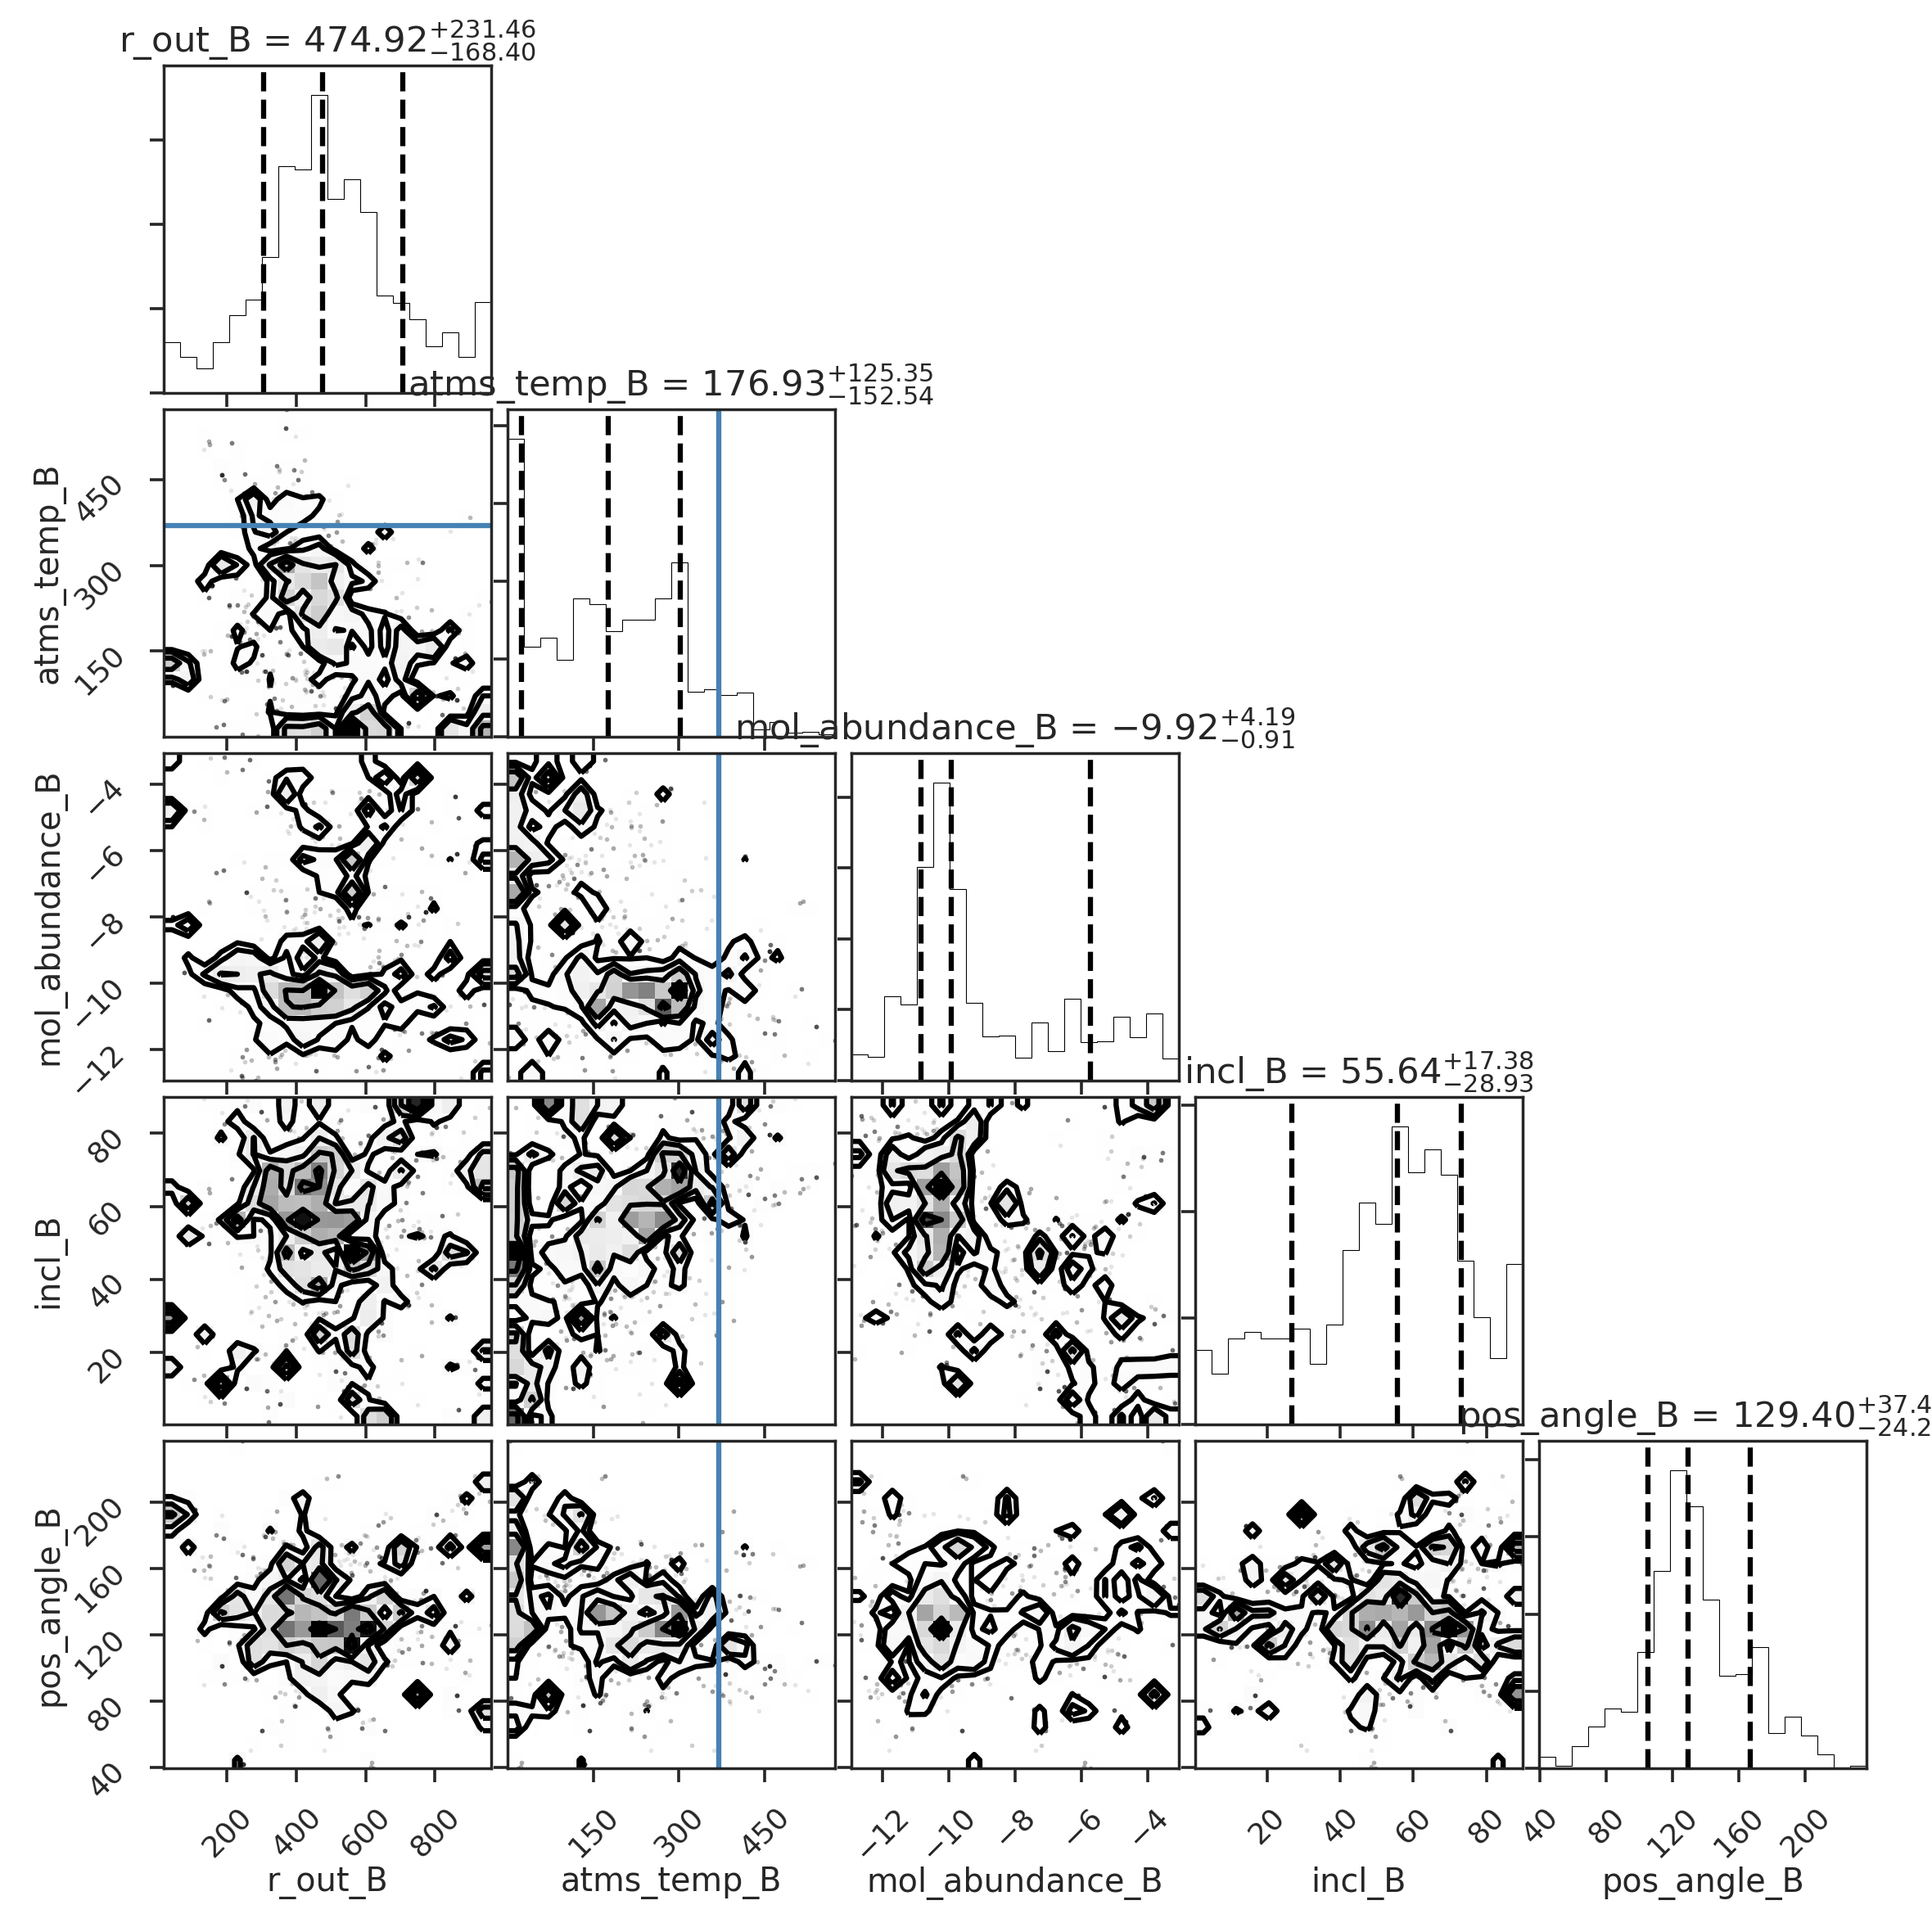
\includegraphics[width=0.49\linewidth]{cornerplot-diskB.png}}%
  \hspace*{\fill}%
  \caption{Since disk A and B's features are assumed to be independent, we may generate corner plots for each of their parameter spaces individually. Some analysis REWORK when new plots are added.}
  \label{fig:corner_plots}
\end{figure}





\section{Fitting Procedure}
\label{section:fitting_procedure}

Fitting of the data began with the analysis and partial removal of cloud contamination discussed in Section \ref{chap:results}, resulting in the removal of baselines below a characteristic length for each line. With the data as clean as possible, position ($\alpha, \delta$) and velocity ($v_\text{sys}$) offsets were fit for. Offset fitting was executed only in the HCO$^+$ line, thanks to the line's minimal contamination and high signal strength. To fit these offsets, all other disk parameters were fixed at hand-selected, ballpark-reasonable values and a grid search was run over RA/Dec offsets and systemic velocities for each disk, using grid resolutions that corresponded to our observation's spectro-spatial resolution. These grids were centered at values drawn from \cite{Williams2014}, where fits were made to the disks' continuum emission, but which proved to be in minor disagreement with our fitting. Positional offsets were confirmed with elliptical Gaussians in \texttt{CASA}. With these values established, they were treated as fixed parameters for the remainder of the fitting process.

% REWORK: Sam includes specific grid resolution and full disk coordinates. Maybe do that here, too.

Table \ref{table:fixed_params} presents a list of parameters, including $\alpha, \delta$, and $v_\text{sys}$, which were left fixed throughout the MCMC runs. Since we are only modeling one line at a time, we are unable to constrain the vertical temperature structure and so fix T$_\text{mid}$ and $z_q$. The selection of midplane temperature was made following \citet{Factor2017} to reflect the "CO snow line" shown by \citet{Qi2011}\footnote{Although their measurements were made for sources in a different environment, the value gives us a reasonable starting point for our fits.}, while the value of $z_q$ was chosen, again following \citet{Factor2017}, to be roughly double the disks' scale heights, as shown in \citet{Rosenfeld2013}. Since HCO+ is optically thin, temperature and density are degenerate, so $\gamma$ is set at 1 following \cite{Andrews2009}, who showed this to be a reasonable value for disks in $\rho$ Ophiuchus. Since our observations do not have enough spectral resolution to constrain the observations' turbulent linewidth, we fix $v_turb$ at around 1\% of the sound speed, per \citet{Williams2014}.


\begin{table}
  \begin{threeparttable}
    \centering
    \caption{Fixed Parameter Values}
    \label{table:fixed_params}
    \renewcommand{\arraystretch}{1.2}
    \begin{tabular}{l  l  l  c  c }
      \toprule \toprule
      \multirow{2}{*}{Parameter} & \multirow{2}{*}{Description} & \multirow{2}{*}{Source} & \multicolumn{2}{c}{Fixed Value(s)} \\
                                 &                              &                         & (Disk A & Disk B) \\
      \midrule %\midrule
      $\Delta \alpha$ ($''$)       &  RA offset from image center     & Grid-search, elliptical fit & 0.0002 & -1.006  \\
      $\Delta \delta$ ($''$)       &  Dec offset from image center    & Grid-search, elliptical fit & 0.082  & -0.3 \\
      v$_\text{sys}$ (km s$^{-1}$) &  Systemic velocity               & Grid-search            & 10.00  & 10.75      \\
      $i$ (\textdegree)            &  Inclination                     & \cite{Williams2014}    & 65 & 45      \\
      M$_\star$ (M$_\odot$)        &  Stellar mass                    & \cite{Williams2014}    & 3.5    & 0.4   \\
      v$_\text{turb}$ (km s$^{-1}$) &  Turbulence velocity             & \cite{Flaherty2015}    & \multicolumn{2}{c}{0.081}   \\
      $d$ (pc)                     &  Distance                        & \cite{GaiaCollaboration2018} & \multicolumn{2}{c}{389}   \\
      R$_c$ (au)                   &  Critical radius                 & \cite{Williams2014}    & \multicolumn{2}{c}{100}\\
      $\gamma$                     &  Radial density power law index} & \cite{Andrews2009}    &  \multicolumn{2}{c}{1}\\
      $z_q$ (au)                   &  Disk scale height at 150 AU     & \cite{Factor2017}          & \multicolumn{2}{c}{29}\\
      T$_\text{mid}$ (K)           &  Midplane temperature at 150 AU  & \cite{Qi2011}          & \multicolumn{2}{c}{19}\\
      \bottomrule
    \end{tabular}

    % \begin{tablenotes}\footnotesize
    %   \item[a] Fit with grid search.
    %   \item[d] Values used by \cite{Flaherty2015} for modeling HD 163296.
    %   \item[e] Retrieved from \cite{Williams2014}
    % \end{tablenotes}
  \end{threeparttable}
\end{table}


The remaining parameters, presented and discussed in \ref{table:fit_params}, are fit for using MCMC. We implement priors on each parameter, reported in Table \ref{table:fit_priors}. Gaussian priors are used for the fitting of both disks' position angles, centered at values presented by \cite{Williams2014}, but which we would like to improve upon.

\begin{table}
  \begin{threeparttable}
    \centering
    \caption{Fit Parameter Values}
    \label{table:fit_priors}
    \renewcommand{\arraystretch}{1.2}
    \begin{tabular}{l  l l }
      \toprule \toprule
      Parameter             &  Description                                     & Prior   \\
      \midrule %\midrule
%      $PA$ ($^o$)           &  Position Angle                                  & Gaussian \\
      X$_\text{mol}$        &  Molecular abundance, relative to H$_2$\tnote{b} & Uniform \\
      $q$                   &  Radial temperature power law index              & Uniform \\
      T$_\text{atms}$ (K)   & Atmosopheric temperature at 150 AU               & Uniform \\
      M$_\text{Disk}$ (M$_\odot$) &  Log Disk mass\tnote{c}                    & Log Uniform \\
      \bottomrule
    \end{tabular}

    \begin{tablenotes}\footnotesize
      %\item[a] Since disk B is unresolved, we fix $i_B = 45$.
      \item[a] For the CO line, X$_\text{mol}$ is fixed at the literature value of $10^{-4}$.
      \item[b] For HCO$^+$(4-3), HCN, and CS, disk mass was fixed at values from \cite{Williams2014}.
    \end{tablenotes}
  \end{threeparttable}
\end{table}


The result from the MCMC runs are presented below. To facilitate easier reading, figures are found at the end of the chapter.

\textit{Note: Everything below here is written kinda just as space filler, based off of the first ~120 steps of each of the three fits. Still, if you could edit as though it is complete, I think that would be helpful for me to see, since I don't really know what I'm doing here!}



\subsection{HCO$^+$ (4-3) Fit}

We began by fitting the HCO+ line, using the MCMC methods explained above.

Best fit and median values with 1-$\sigma$ uncertainties are given in Table \ref{table:fit_hco}, while corner plots, showing the posterior distributions of the individual line fit, is shown in Fig. \ref{fig:hco_corner_plots}. The corner plot shows that all parameters are fairly well constrained. I actually don't really see any degeneracies here?

Channel maps showing the data, best-fit model, and data-model residuals are shown in Fig. \ref{fig:co_chanmaps}. Some residuals probably exist, and they probably line up with the CO contamination.


\begin{table}
  \centering
  \begin{threeparttable}
    \caption{MCMC Fitting Results (HCO$^+$)}
    \label{table:fit_hco}
    \renewcommand{\arraystretch}{1.2}
    \begin{tabular}{c c l c l }
      \toprule \toprule
      %\multirow{2}{*}{Parameter} & \multirow{2}{*}{Disk A}    & \multicolumn{2}{c}{Disk B} \\
      \multirow{2}{*}{Parameter} & \multicolumn{2}{c}{Disk A} & \multicolumn{2}{c}{Disk B} \\
                                 & Median & Best Fit          & Median & Best Fit \\
      \midrule %\midrule
      X$_\text{mol}$            & $ -n _{-0.} ^{+0.}$ & $-8.12$    & $ -n _{-0.} ^{+0.}$ & $-10.3$ \\
      $r_{out}$(\si{au})        & $ -n _{-0.} ^{+0.}$ & $333.86$    & $ -n _{-0.} ^{+0.}$  & $240.69$    \\
      $i$ (\si{\degree})        & $ -n _{-0.} ^{+0.}$ & $[65]$    & $ -n _{-0.} ^{+0.}$ & $[45]$    \\
      PA  (\si{\degree})        & $ -n _{-0.} ^{+0.}$ & $69.79$  & $ -n _{-0.} ^{+0.}$  & $121.22$  \\
      q                         & $ -n _{-0.} ^{+0.}$ & $0.77$  & $ -n _{-0.} ^{+0.}$  & $[-0.5]$  \\
      T$_\text{atms}$ (\si{\K}) & $ -n _{-0.} ^{+0.}$ & $172.95 $  & $ -n _{-0.} ^{+0.}$  & $183.17$  \\
      lnprob                    & \multicolumn{4}{c}{$-28404.97$} \\
      \bottomrule
    \end{tabular}
    \begin{tablenotes}\footnotesize
      \item[*] Values in [brackets] were fixed for this run.
    \end{tablenotes}
  \end{threeparttable}
\end{table}








\subsection{HCN (4-3) Fit}

We proceed by next modeling HCN, following a similar path to the one taken for CO. As before, best fit and median values with 1-$\sigma$ uncertainties are given in Table \ref{table:fit_hcn}, channel maps are presented in Fig. \ref{fig:hcn_chanmaps}, and corner plots are shown in Fig. \ref{fig:hcn_corner_plots}.

In this run, we fix both disk's position angles at % REWORK: Figure out who

For this line, the plots show that, while the solutions are generally unimodal, there are significant degeneracies between parameters. Most notable amongst these are the relationships between disk B's outer radius and its atmospheric temperature, molecular abundance, and position angle. These degeneracies are, in some sense, to be expected, since the disk is not resolved and so the MCMC struggles to differentiate between flux contributors.

A slightly more interesting pattern is found in the relationship betwen disk B's outer radius and disk A's atmospheric temperature, molecular abundance, temperature structure, and outer radius. This may be the result of the MCMC trying to make sense of the potential tidal feature linking the two disks, which is particularly noticeable in the HCN channel maps (relative to HCO+ and CO). The bimodal hump in disk B's outer radius is a bit of a mystery to me, unless it represents the walkers' deciding to commit to either fitting or not fitting the tidal feature.



% Note: Maybe use pd.df.to_latex() to populate these tables?
\begin{table}
  \begin{threeparttable}
    \centering
    \caption{MCMC Fitting Results (HCN)}
    \label{table:fit_hcn}
    \renewcommand{\arraystretch}{1.2}
    \begin{tabular}{c c l c l }
      \toprule \toprule
      %\multirow{2}{*}{Parameter} & \multirow{2}{*}{Disk A}    & \multicolumn{2}{c}{Disk B} \\
      \multirow{2}{*}{Parameter} & \multicolumn{2}{c}{Disk A} & \multicolumn{2}{c}{Disk B} \\
                                 & Median & Best Fit          & Median & Best Fit \\
      \midrule %\midrule
      X$_\text{mol}$             & $ -n _{-0.} ^{+0.}$ & $-7.87$    & $ -n _{-0.} ^{+0.}$ & $-11.09$ \\
      $r_{out}$(\si{au})        & $ -n _{-0.} ^{+0.}$ & $334.48$    & $ -n _{-0.} ^{+0.}$  & $292.37$    \\
      $i$ (\si{\degree})        & $ -n _{-0.} ^{+0.}$ & $[65]$   & $ -n _{-0.} ^{+0.}$ & $[45]$    \\
      PA  (\si{\degree})        & $ -n _{-0.} ^{+0.}$ & $70.05$  & $ -n _{-0.} ^{+0.}$  & $134.2$  \\
      q                         & $ -n _{-0.} ^{+0.}$ & $0.62$  & $ -n _{-0.} ^{+0.}$  & $[-0.5]$  \\
      T$_\text{atms}$ (\si{\K}) & $ -n _{-0.} ^{+0.}$ & $125.68 $  & $ -n _{-0.} ^{+0.}$  & $388.21$  \\
      $\ln$ Likelihood          & \multicolumn{4}{c}{$-30928.35$} \\
      \bottomrule
    \end{tabular}
    \begin{tablenotes}\footnotesize
      \item[*] Values in [brackets] were fixed for this run.
    \end{tablenotes}
  \end{threeparttable}
\end{table}





\subsection{CO(3-2) Fit}
We began by fitting the CO line. Since we fix CO's relative molecular abundance at X$_\text{mol}=10^{-4}$, we may directly fit for the disks' masses and then use those values for the other lines.

The significant cloud contamination in the CO line presents difficulties for fitting. Since the contamination is most significant in the central five channels, those channels were not included in the fitting process. Although this degrades the

Additionally, maybe a tidal feature. Best fit values are reported in Table \ref{table:fit_co}


Finally, we fit the CO(3-2) line. Fit results are summarized in \ref{table:fit_co}, and visualized in \ref{fig:co_corner_plots} and \ref{fig:co_chanmaps}.


Despite the removal of baselines below 60 k$\lambda$, the CO(3-2) line still shows significant cloud contamination in channels near the systemic velocity. In order to avoid having the MCMC walkers try to fit the contamination, we remove the channels with velocities between 9.88 and 12 km s$^{-1}$, which show the worst of the contamination. By choosing to not include these, we sacrifice some data, but the resulting fits are more representative of the structures we care about - the disks themselves - than they would be had we not sacrificed those channels.

Still, the resulting fits are noticeably less certain than those of the HCO+ and HCN lines, featuring several bimodal posteriors. Not really sure what to do about this. Manually cut some of them?


\begin{table}
  \begin{threeparttable}
    \centering
    \caption{MCMC Fitting Results (CO)}
    \label{table:fit_co}
    \renewcommand{\arraystretch}{1.2}
    \begin{tabular}{c c l c l }
      \toprule \toprule
      %\multirow{2}{*}{Parameter} & \multirow{2}{*}{Disk A}    & \multicolumn{2}{c}{Disk B} \\
      \multirow{2}{*}{Parameter} & \multicolumn{2}{c}{Disk A} & \multicolumn{2}{c}{Disk B} \\
                                 & Median & Best Fit          & Median & Best Fit \\
      \midrule %\midrule
      $\log M_\text{Disk}$ (M$_\odot$) & $ -n _{-0.} ^{+0.}$ & $-0.29$    & $ -n _{-0.} ^{+0.}$ & $-4.9$ \\
      $r_{out}$(\si{au})               & $ -n _{-0.} ^{+0.}$ & $437.71$    & $ -n _{-0.} ^{+0.}$  & $261.13$    \\
      $i$ (\si{\degree})               & $ -n _{-0.} ^{+0.}$ & $65$    & $ -n _{-0.} ^{+0.}$ & $45$    \\
      PA  (\si{\degree})               & $ -n _{-0.} ^{+0.}$ & $66.73$  & $ -n _{-0.} ^{+0.}$  & $[136]$  \\
      q                                & $ -n _{-0.} ^{+0.}$ & $0.28$  & $ -n _{-0.} ^{+0.}$  & $[-0.5]$  \\
      T$_\text{atms}$ (K)              & $ -n _{-0.} ^{+0.}$ & $5.54 $  & $ -n _{-0.} ^{+0.}$  & $177.15$  \\
      $\ln$ Likelihood          & \multicolumn{4}{c}{$-33597.46$} \\
      \bottomrule
    \end{tabular}

    \begin{tablenotes}\footnotesize
      \item[*] Values in [brackets] were fixed for this run.
    \end{tablenotes}
  \end{threeparttable}
\end{table}








%% ~~~~ FIGURES ~~~~~~~~~~~~~~~~~~~~~~~~~~~~~~~~~~~~~~~~~~~~~~~~~~~~~~~~~~~~~~~~


%% ~~~ HCO ~~~~~~~~~~~~~~~~~~~~~~~~~~~~~~~~~~~~~~~~~~~~~~~~~~~~~~~~~~~~~~~~~~~~~


\begin{figure}[htp]
  \hspace*{\fill}%
  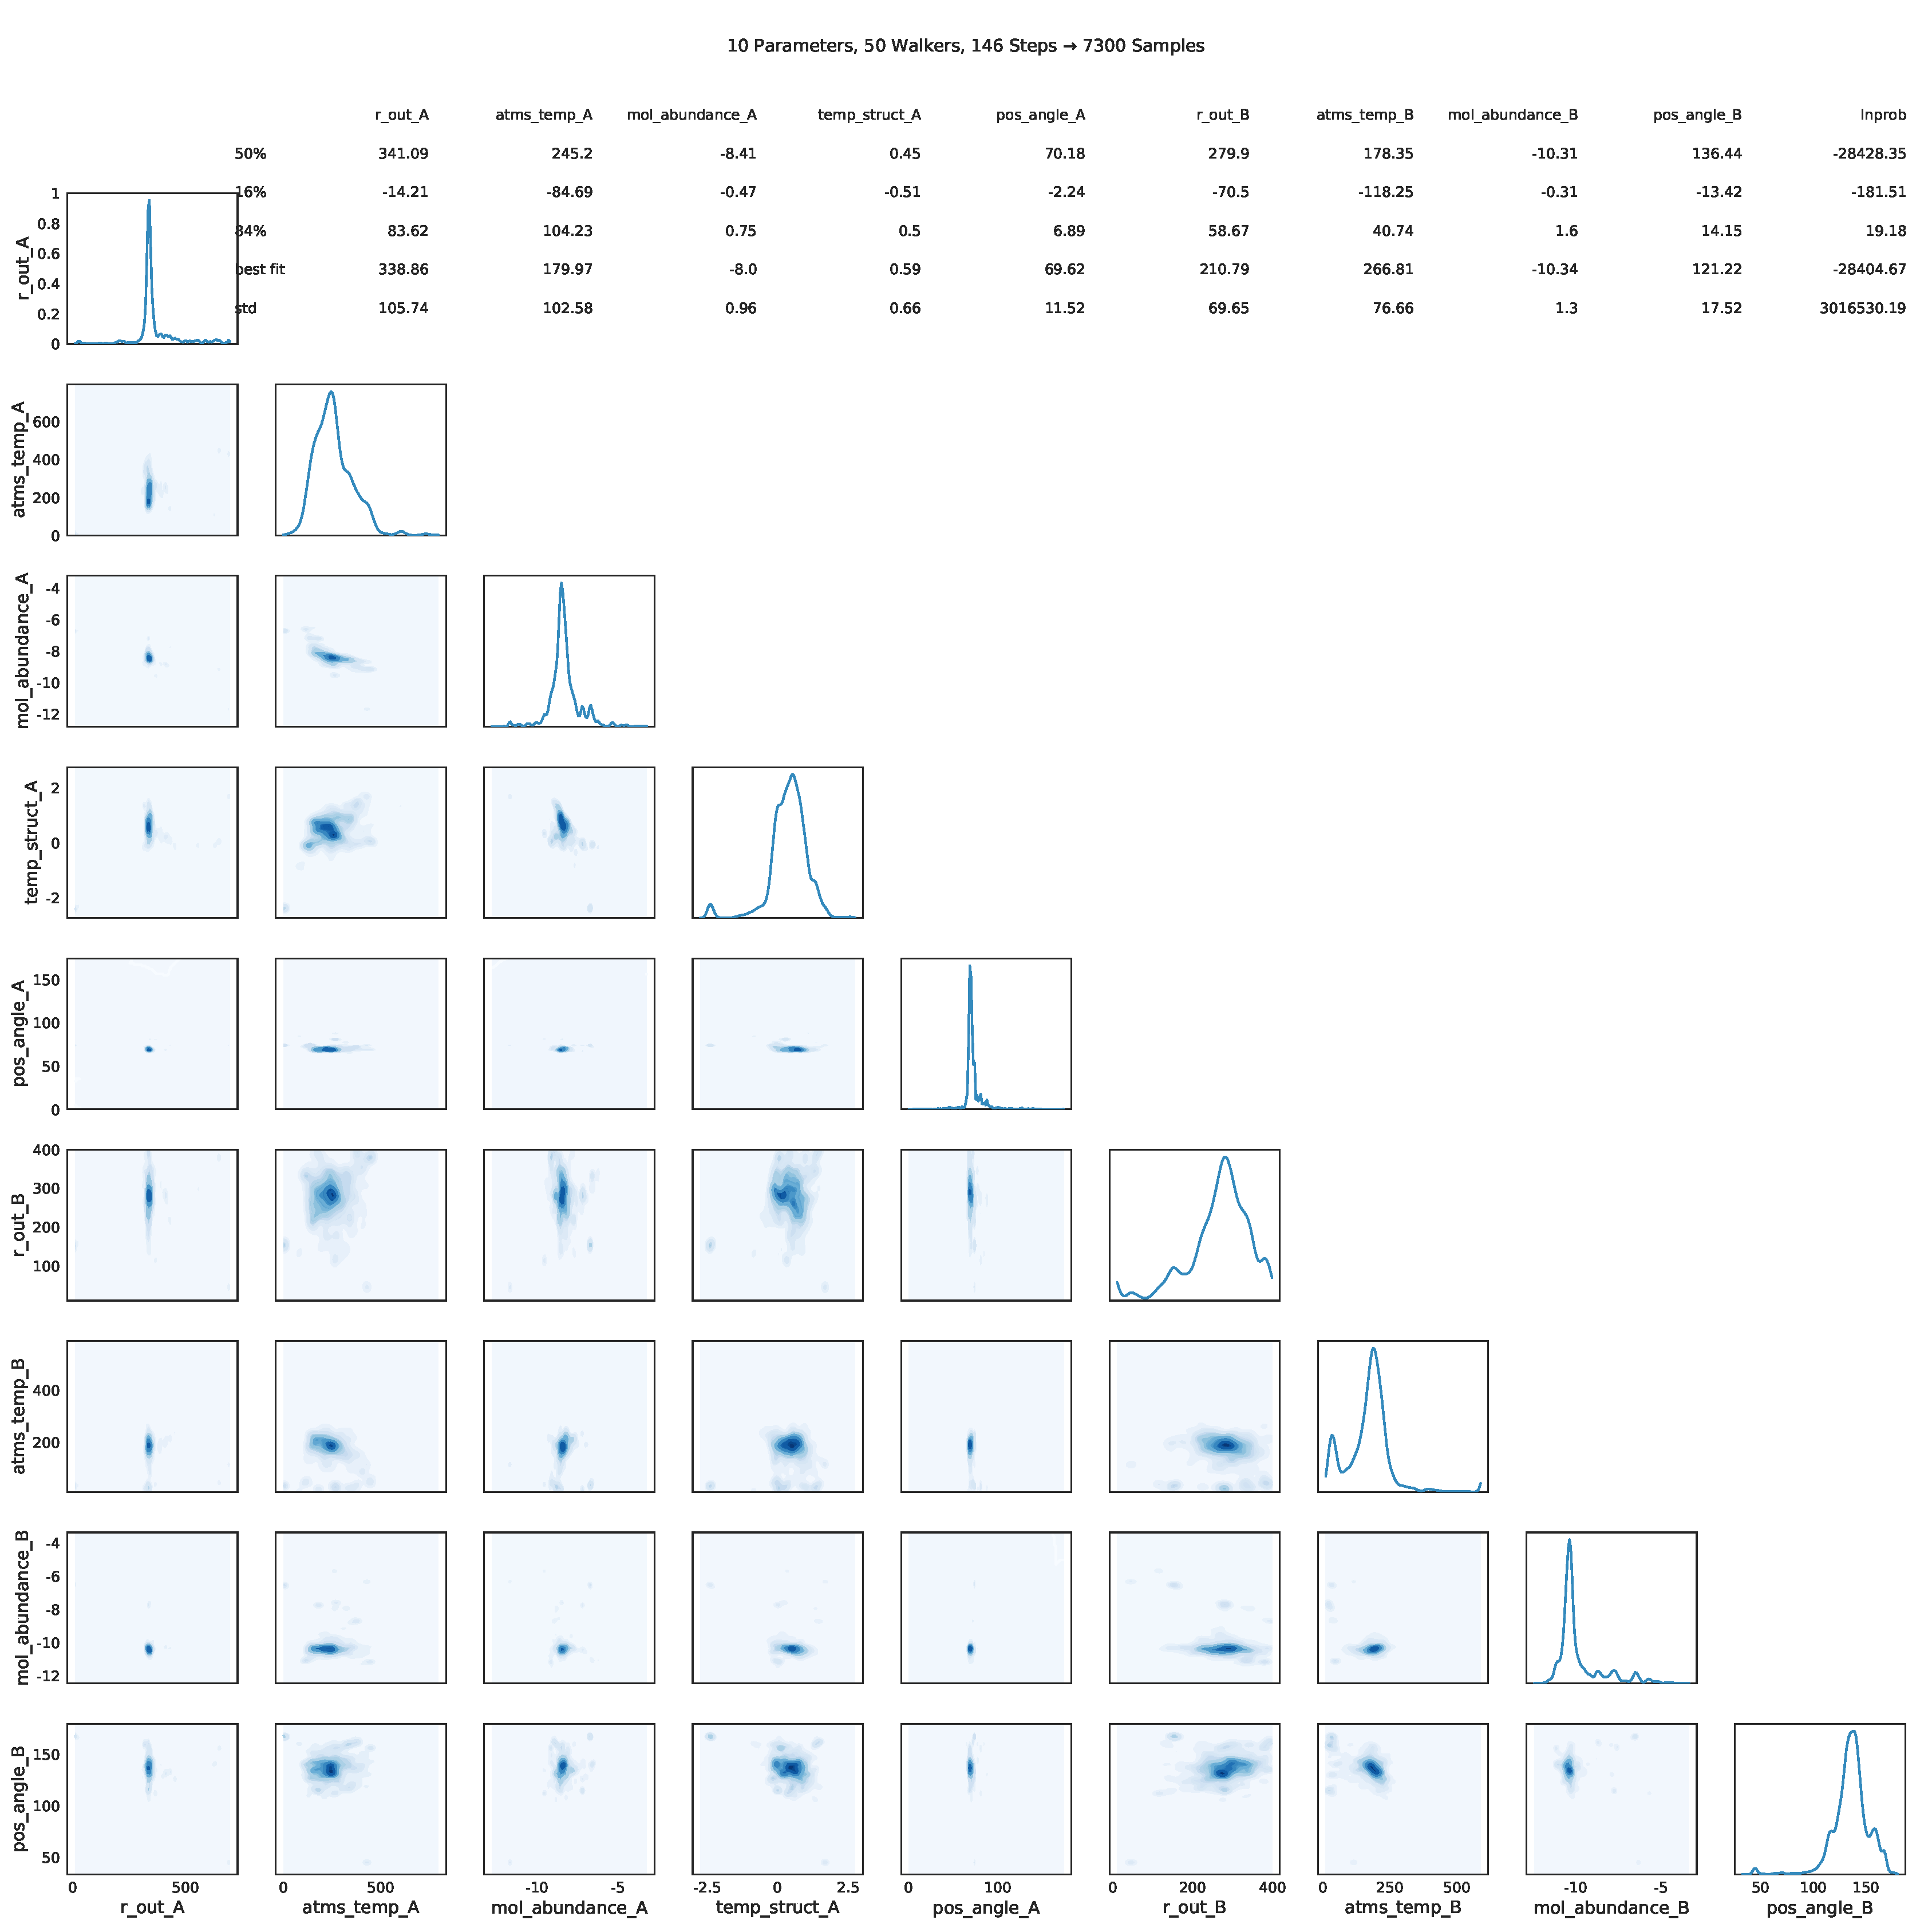
\includegraphics[width=\linewidth]{cornerplots-hco.pdf}\hfill%
  \hspace*{\fill}%
  \caption{Data, model, and residual maps are presented.}
  \label{fig:hco_cornerplots}
\end{figure}



\begin{figure}[htp]
  \hspace*{\fill}%
  \includegraphics[width=\linewidth]{chanmaps-hco.pdf}\hfill%
  \hspace*{\fill}%
  \caption{Data, model, and residual maps are presented.}
  \label{fig:hco_chanmaps}
\end{figure}

%% ~~~ HCN ~~~~~~~~~~~~~~~~~~~~~~~~~~~~~~~~~~~~~~~~~~~~~~~~~~~~~~~~~~~~~~~~~~~~~

\begin{figure}[htp]
  \hspace*{\fill}%
  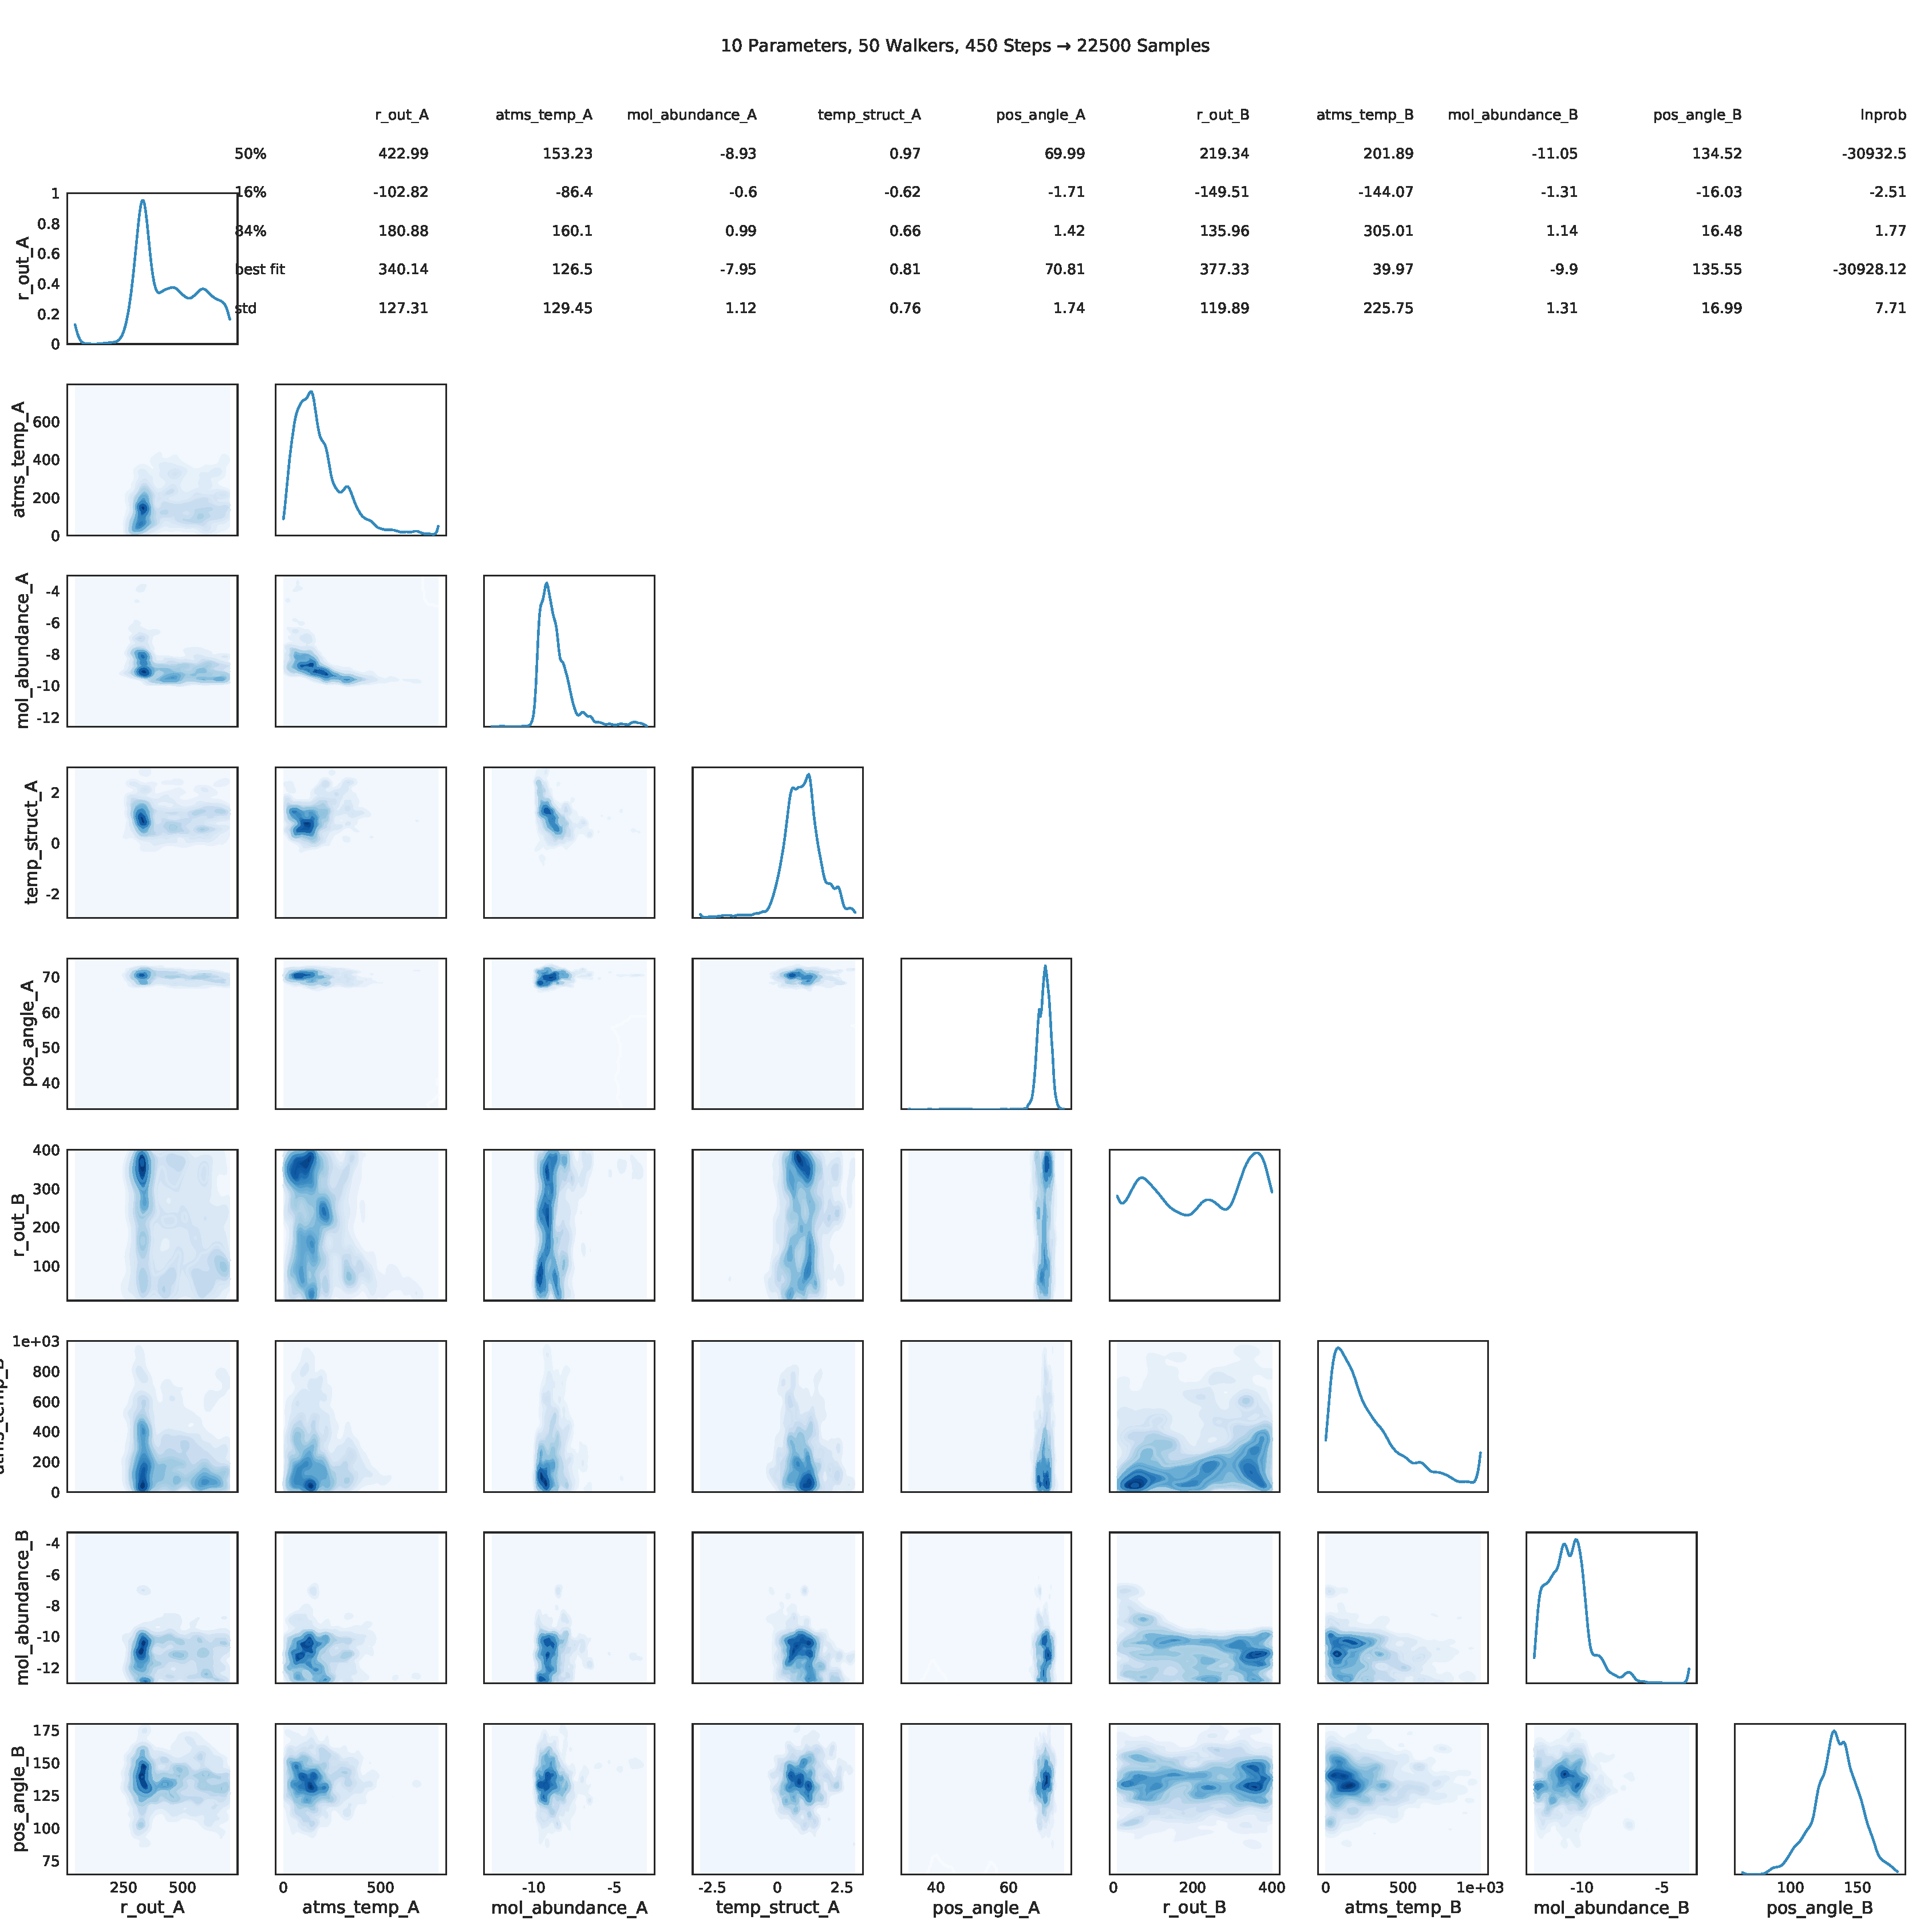
\includegraphics[width=\linewidth]{cornerplots-hcn.pdf}\hfill%
  \hspace*{\fill}%
  \caption{Since disk A and B's features are assumed to be independent, we may generate corner plots for each of their parameter spaces individually. Some analysis REWORK when new plots are added.}
  \label{fig:hcn_cornerplots}
\end{figure}



\begin{figure}[htp]
  \hspace*{\fill}%
  \includegraphics[width=\linewidth]{chanmaps-hcn.pdf}\hfill%
  \hspace*{\fill}%
  \caption{Since disk A and B's features are assumed to be independent, we may generate corner plots for each of their parameter spaces individually. Some analysis REWORK when new plots are added.}
  \label{fig:hcn_chanmaps}
\end{figure}



%% ~~~ CO ~~~~~~~~~~~~~~~~~~~~~~~~~~~~~~~~~~~~~~~~~~~~~~~~~~~~~~~~~~~~~~~~~~~~~~

\begin{figure}[htp]
  \hspace*{\fill}%
  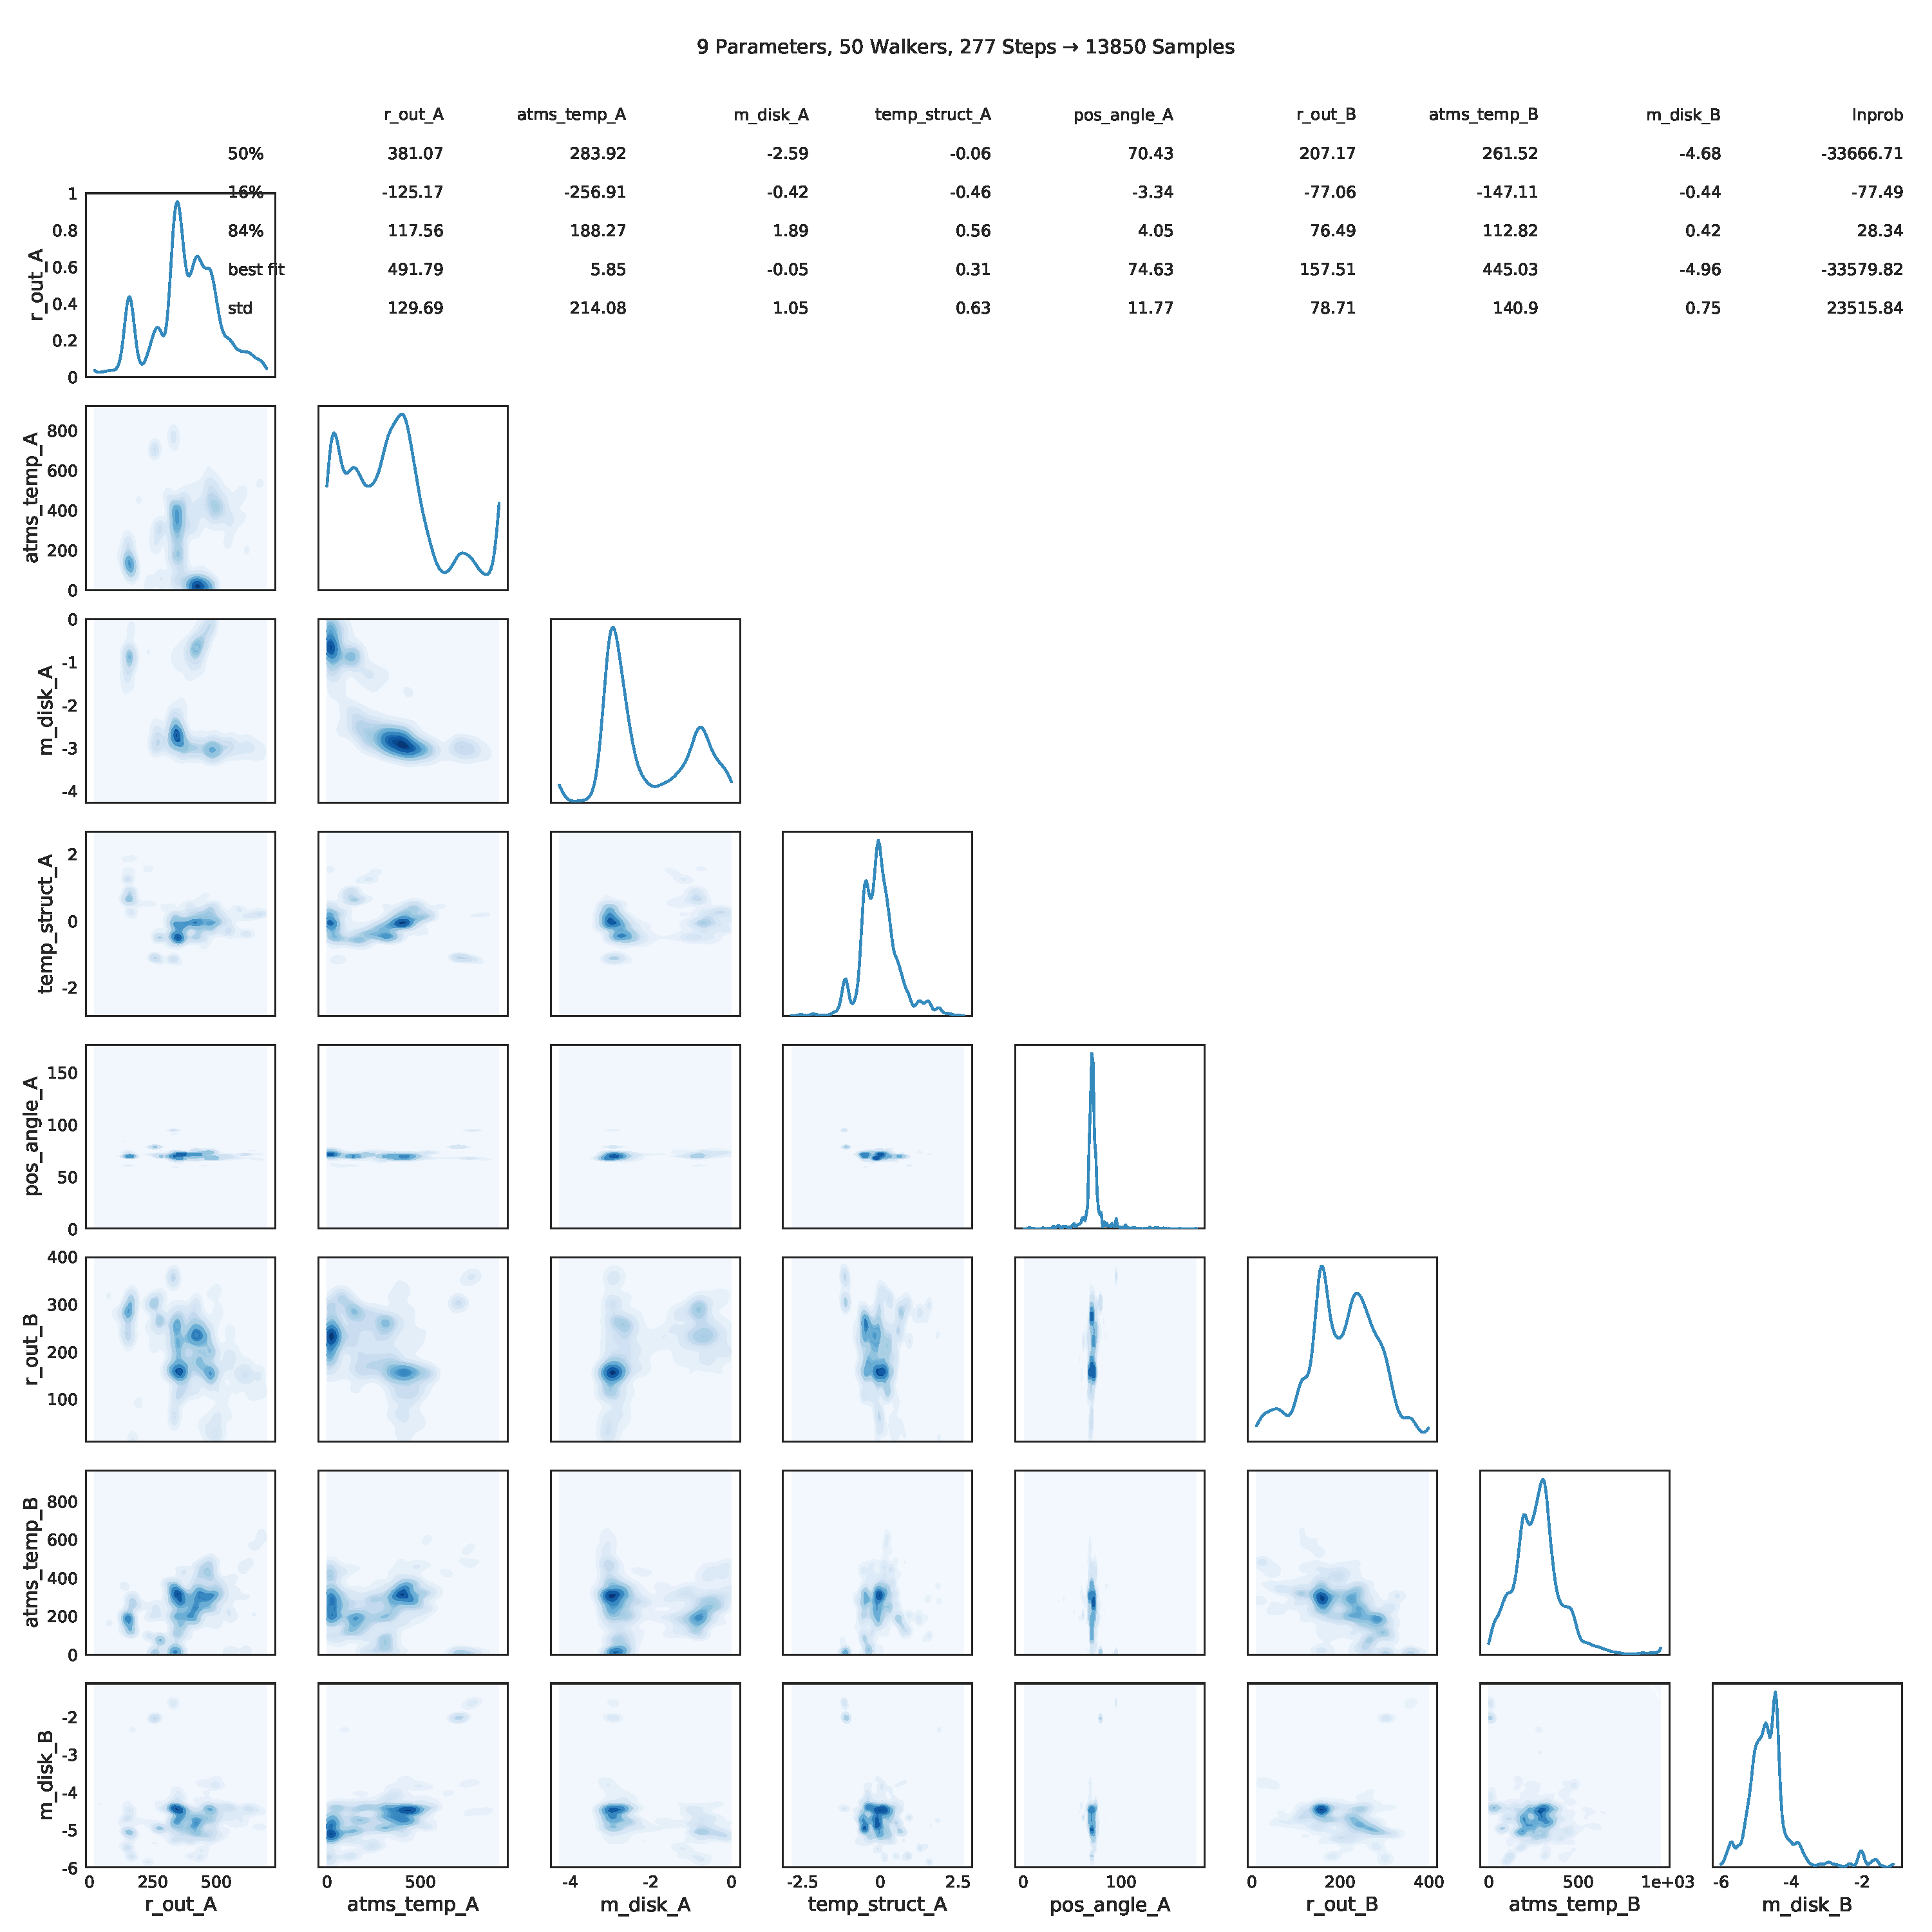
\includegraphics[width=\linewidth]{cornerplots-co.pdf}\hfill%
  \hspace*{\fill}%
  \caption{Since disk A and B's features are assumed to be independent, we may generate corner plots for each of their parameter spaces individually. Some analysis REWORK when new plots are added.}
  \label{fig:co_cornerplots}
\end{figure}


% \begin{figure}[htp]
%   \hspace*{\fill}%
%   \subcaptionbox{Disk A fits \label{fig:corner_a}}{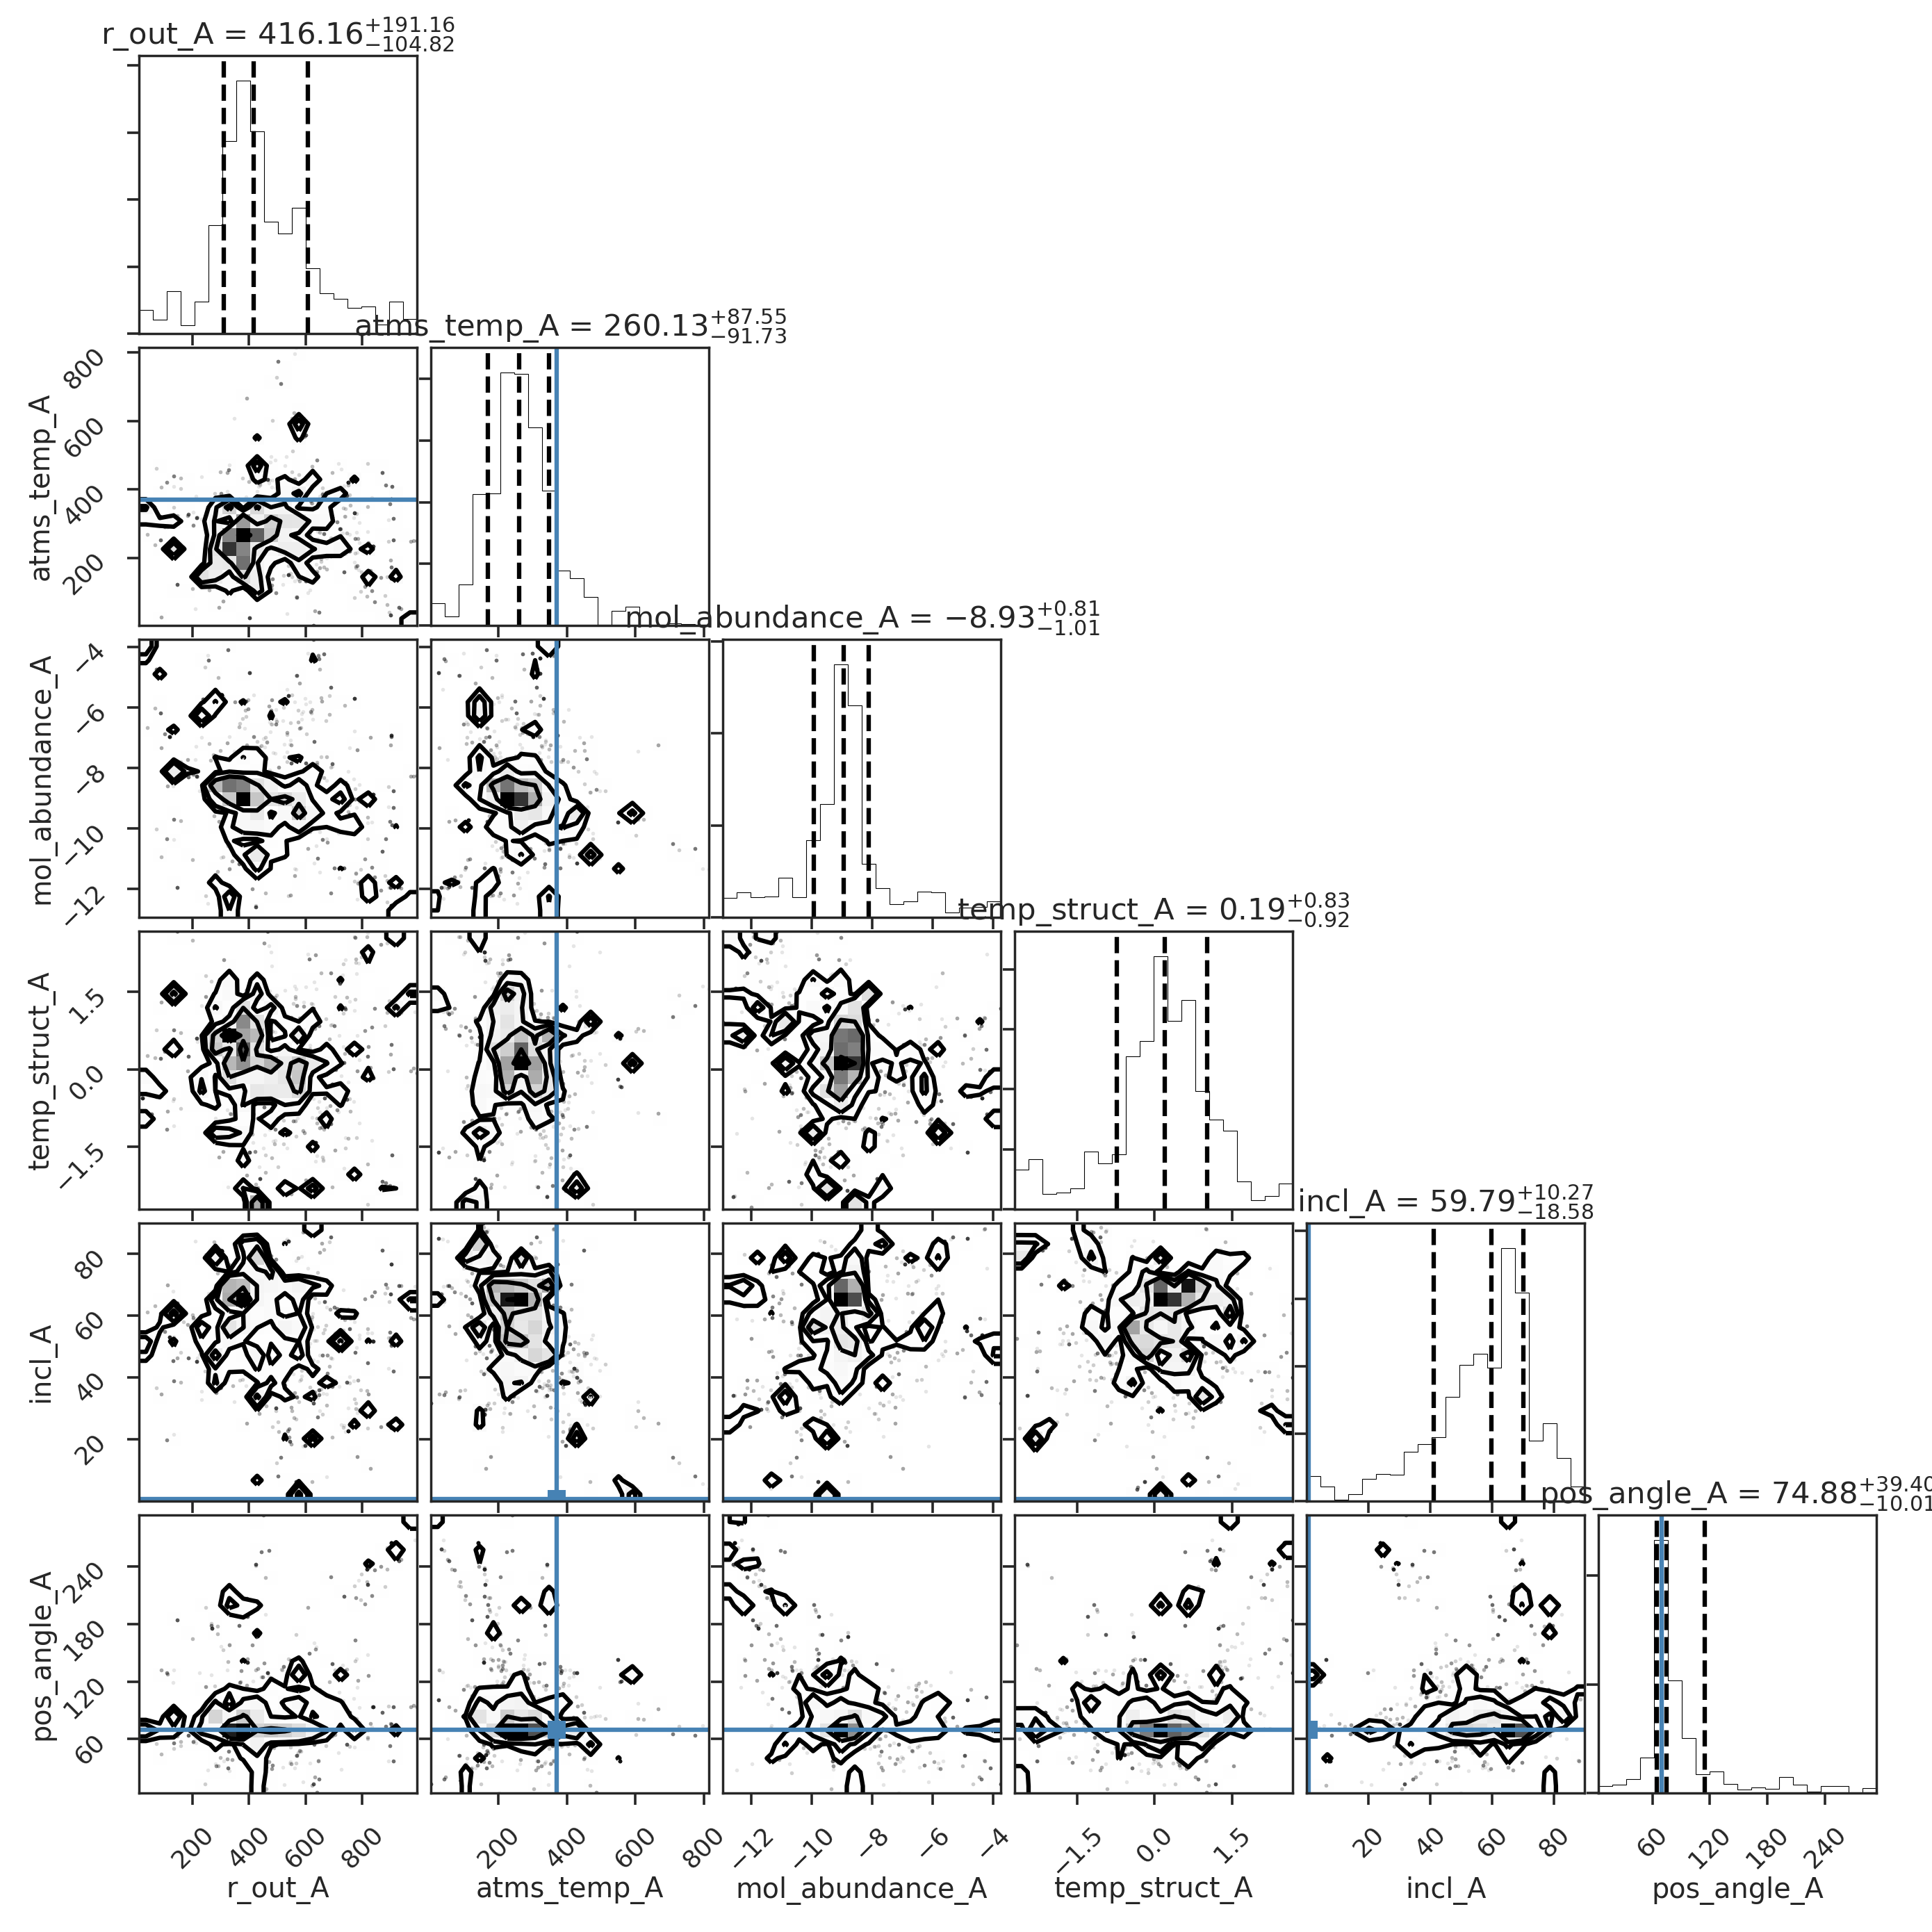
\includegraphics[width=0.49\linewidth]{cornerplot-diskA.png}}\hfill%
%   \subcaptionbox{Disk B fits \label{fig:corner_b}}{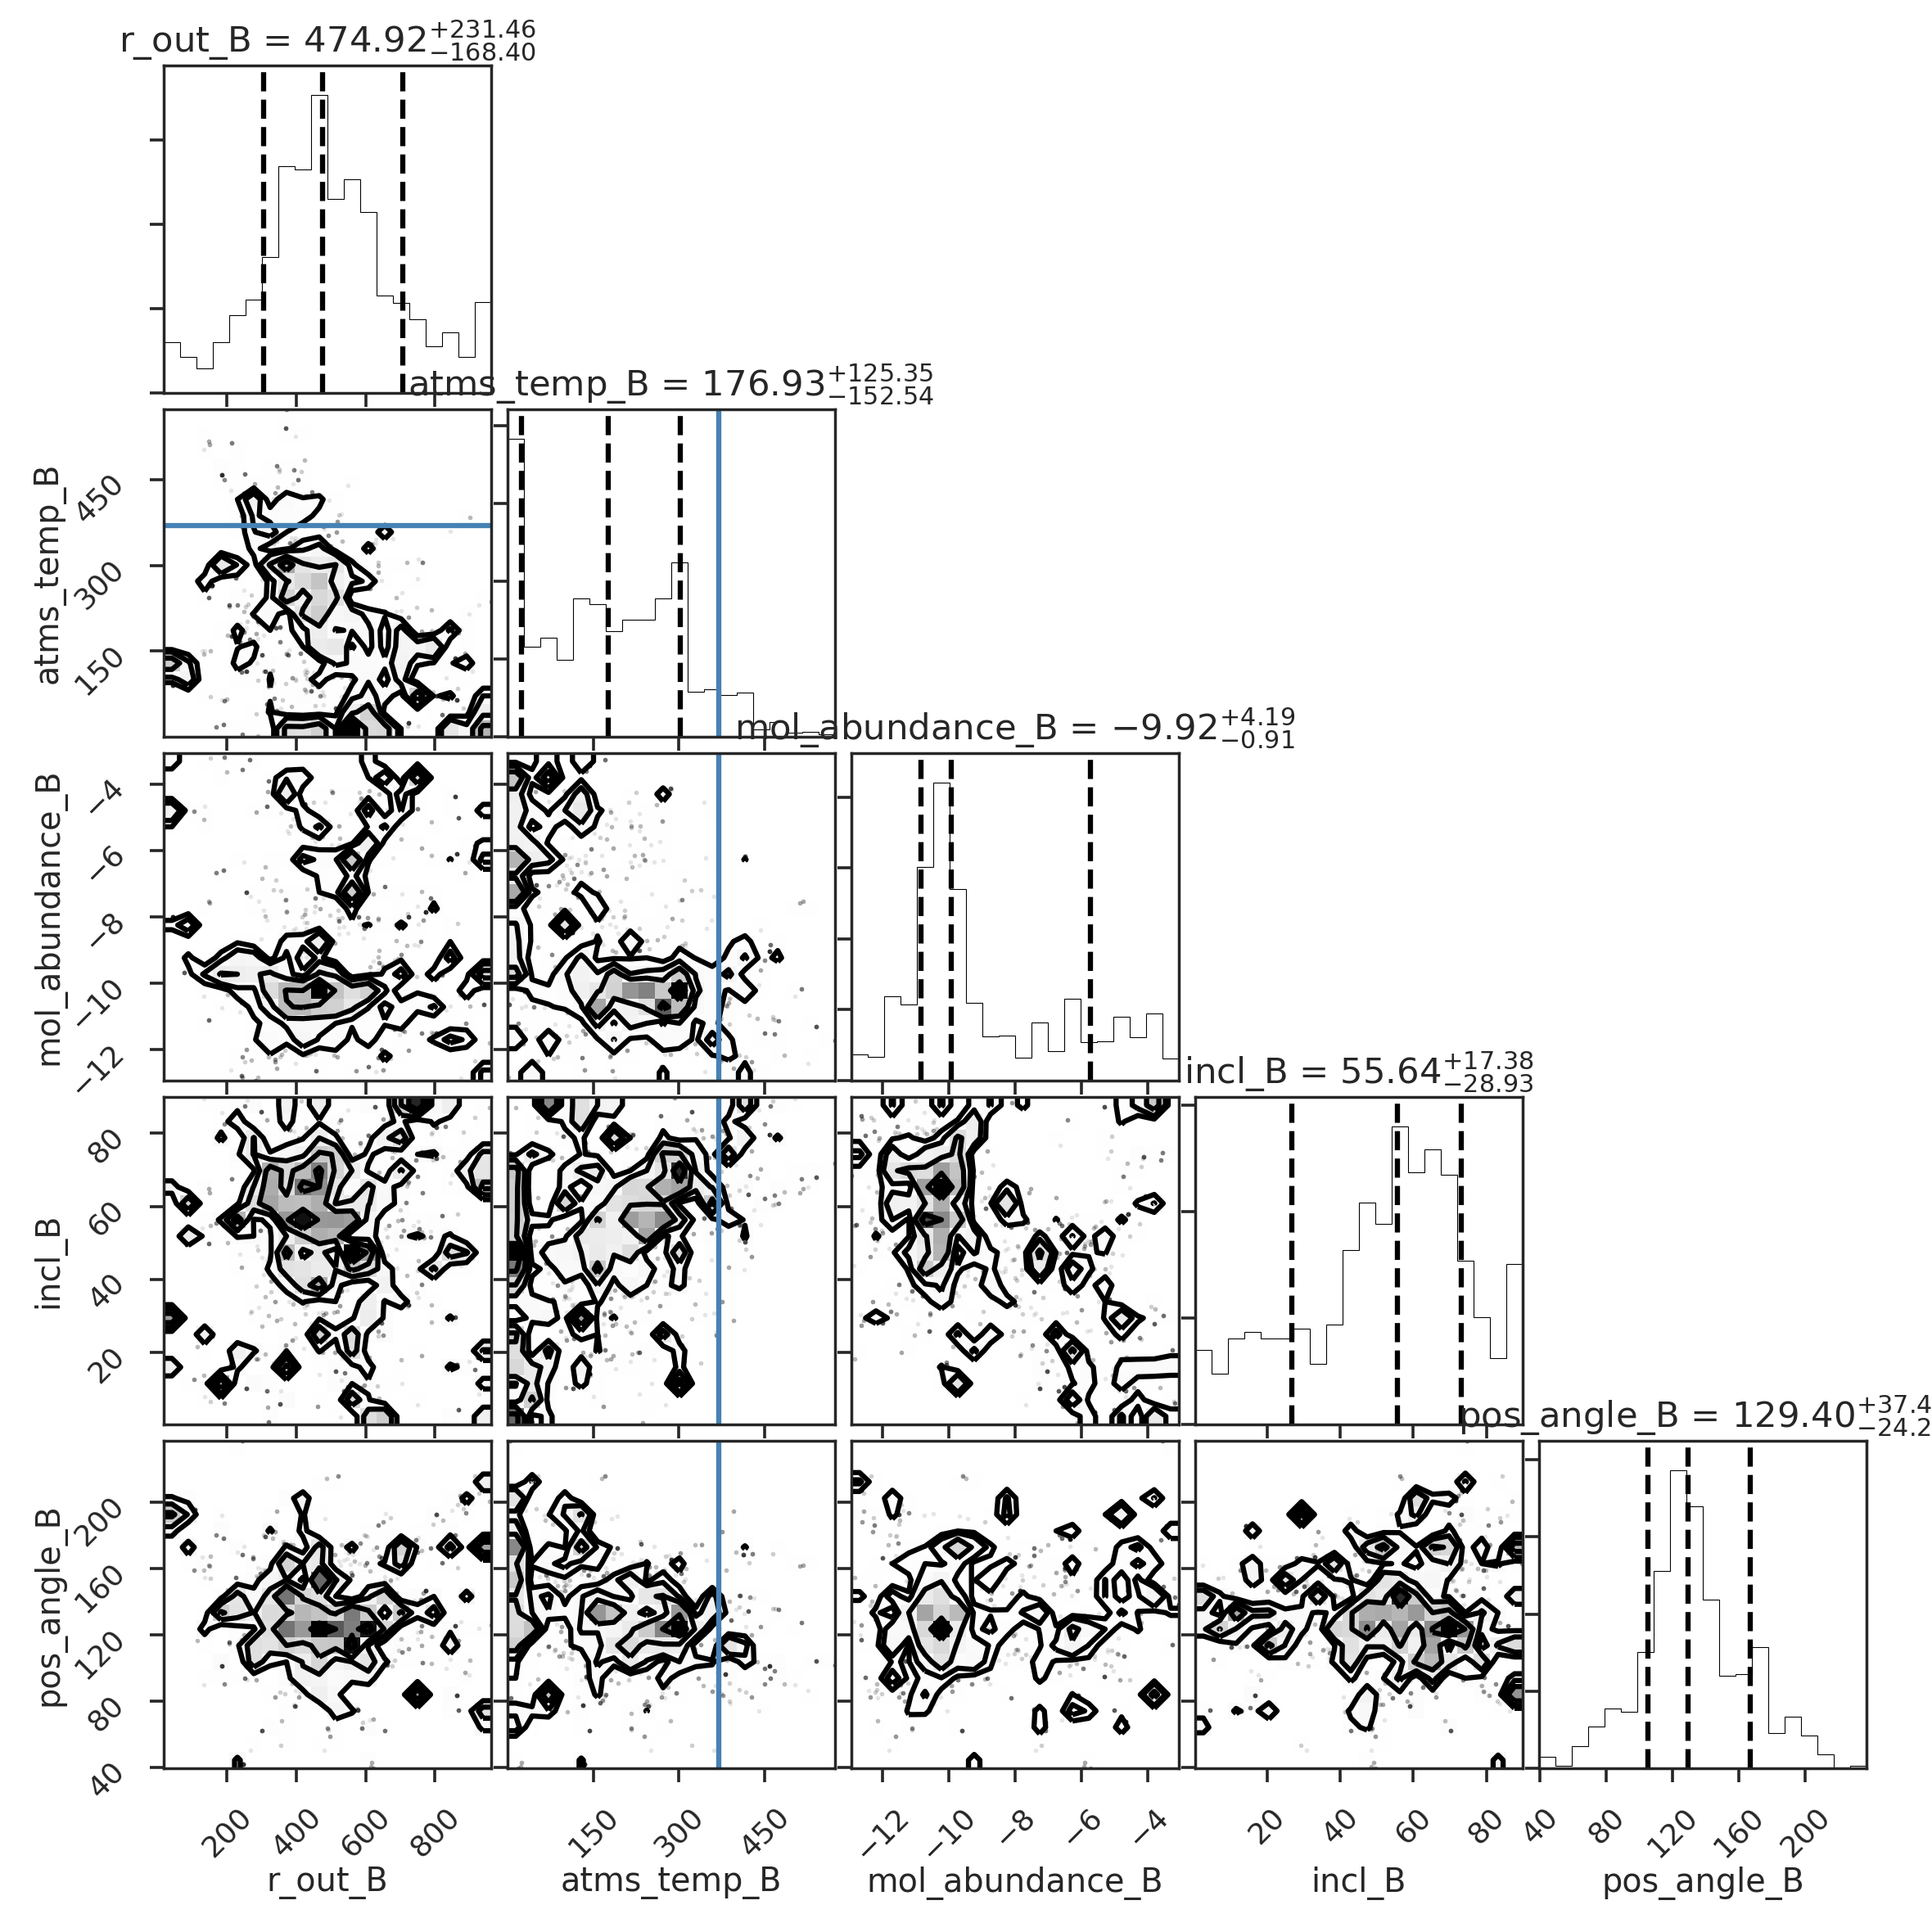
\includegraphics[width=0.49\linewidth]{cornerplot-diskB.png}}%
%   \hspace*{\fill}%
%   \caption{Since disk A and B's features are assumed to be independent, we may generate corner plots for each of their parameter spaces individually. Some analysis REWORK when new plots are added.}
%   \label{fig:co_corner_plots}
% \end{figure}


\begin{figure}[htp]
  \hspace*{\fill}%
  \includegraphics[width=\linewidth]{chanmaps-co.pdf}\hfill%
  \hspace*{\fill}%
  \caption{Since disk A and B's features are assumed to be independent, we may generate corner plots for each of their parameter spaces individually. Some analysis REWORK when new plots are added.}
  \label{fig:co_chanmaps}
\end{figure}






\begin{figure}
  \centering
  \begin{minipage}{.33\textwidth}
    \centering
    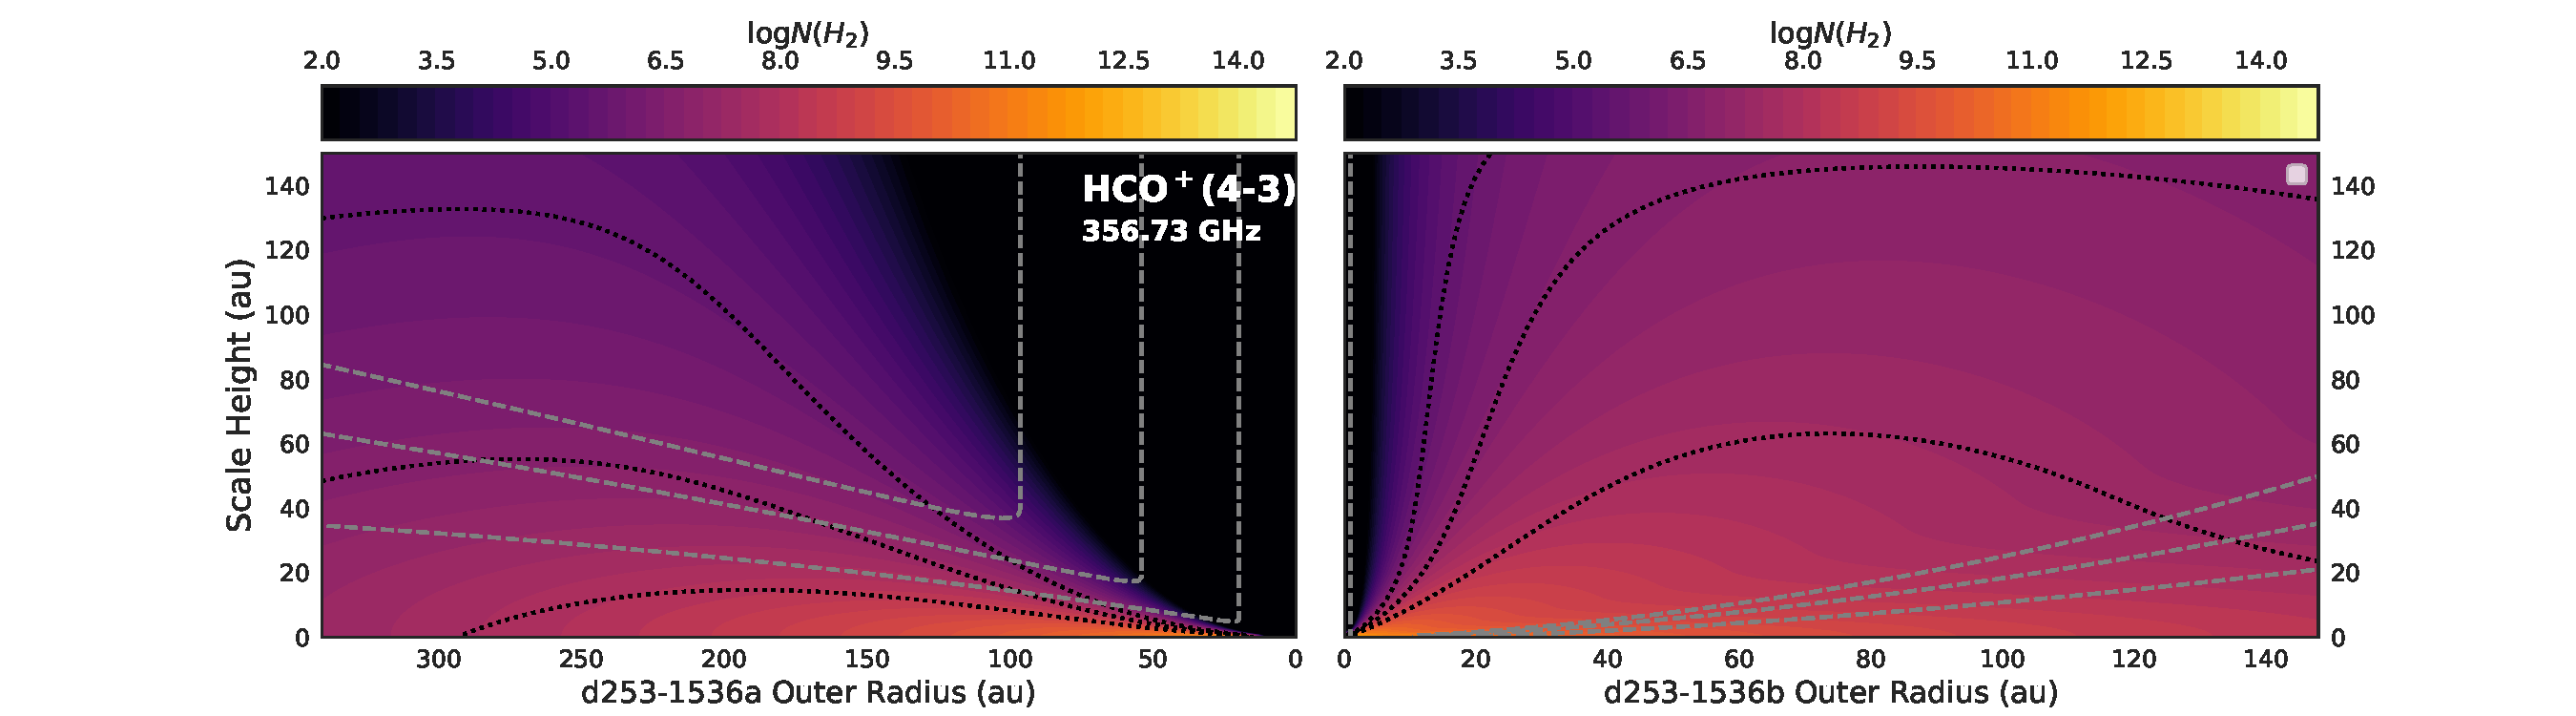
\includegraphics[width=\linewidth]{diskstructures-hco.pdf}
    \captionof{figure}{Disk structure}
    \label{fig:disk_str_hco}
  \end{minipage}%
  \begin{minipage}{.33\textwidth}
    \centering
    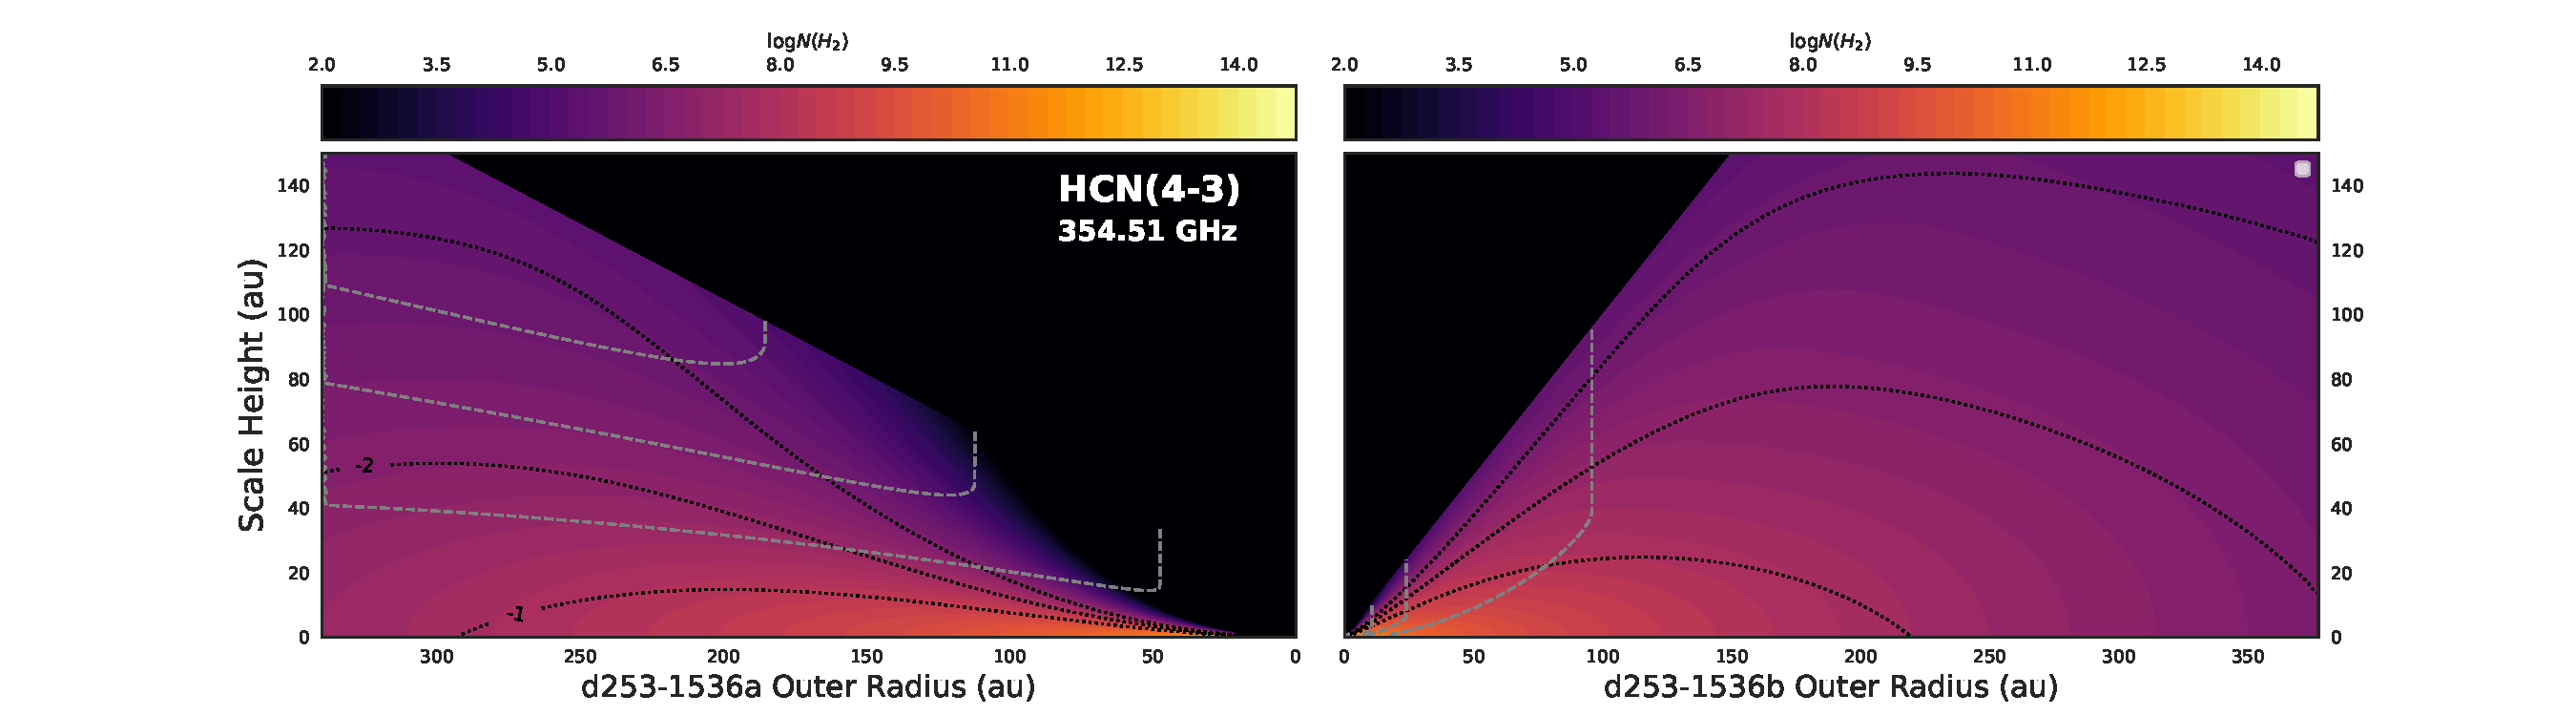
\includegraphics[width=\linewidth]{diskstructures-hcn.pdf}
    \captionof{figure}{Disk structure}
    \label{fig:disk_str_hcn}
  \end{minipage}%
  %\par\medskip
  \begin{minipage}{.33\textwidth}
    \centering
    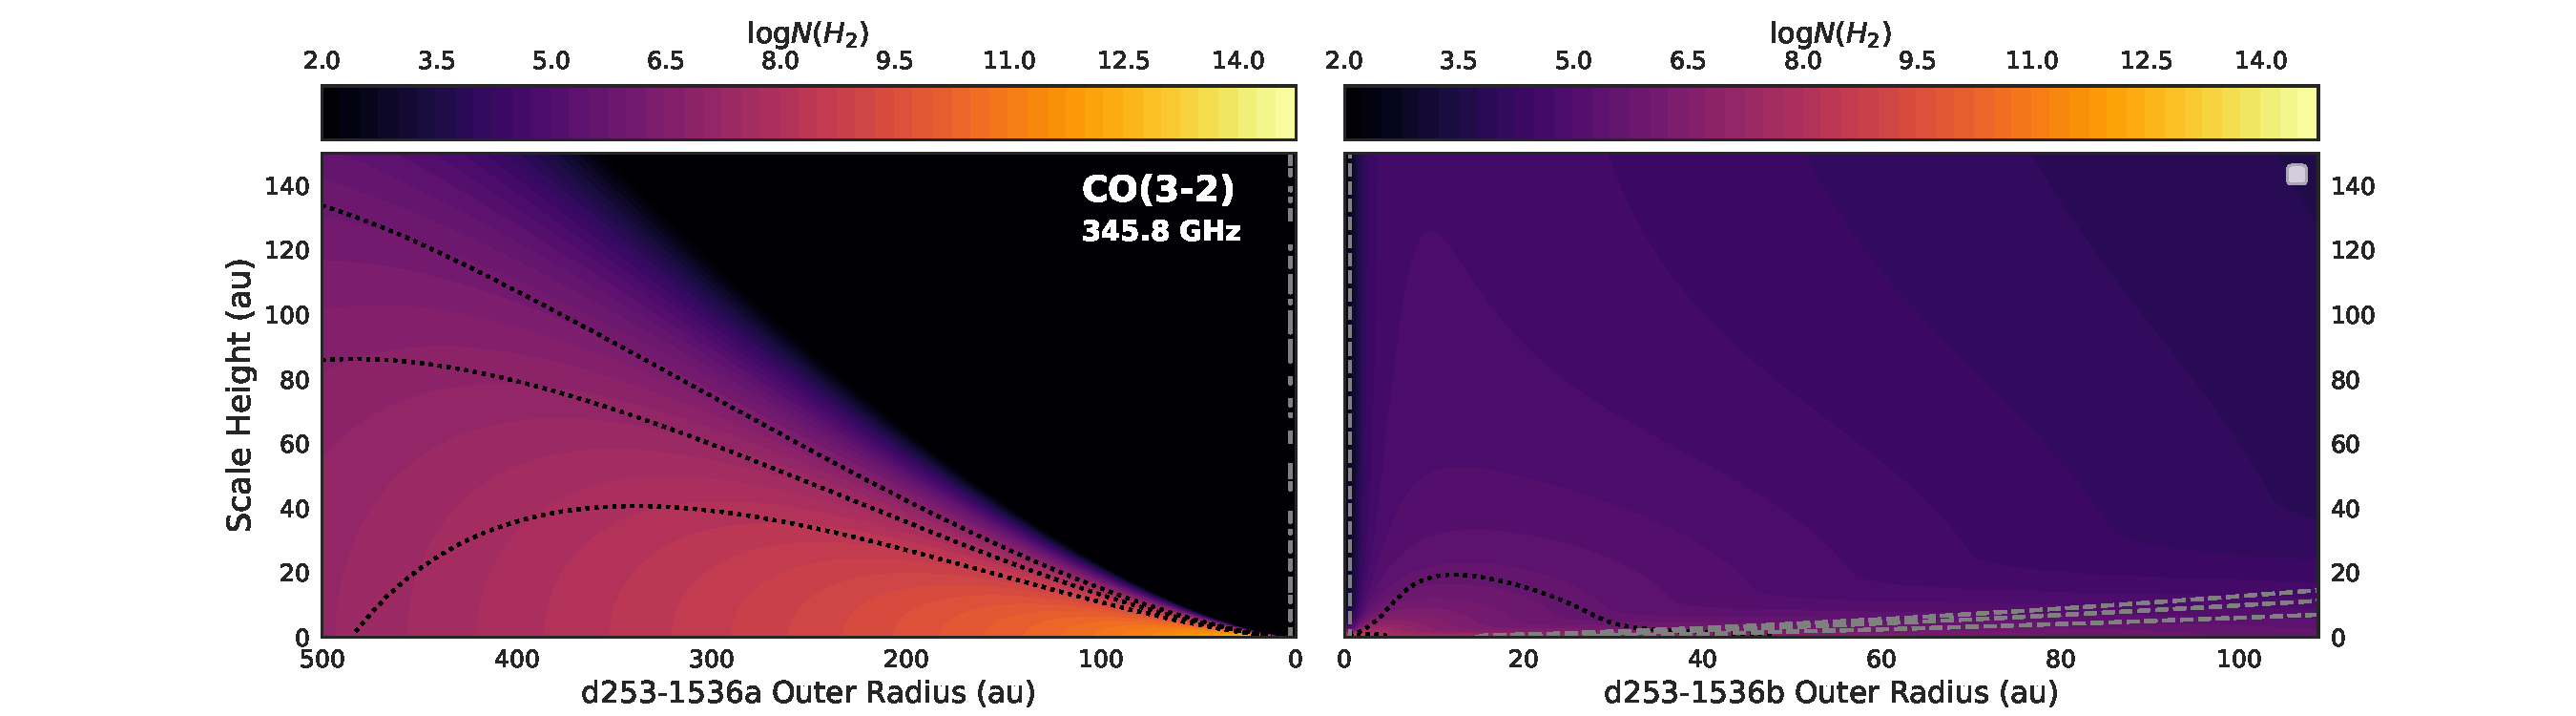
\includegraphics[width=\linewidth]{diskstructures-co.pdf}
    \captionof{figure}{Disk structure}
    \label{fig:disk_str_co}
  \end{minipage}%
  \label{fig:noise-profiles}
\end{figure}


% \begin{itemize}
%   \item \textsc{RA/Dec Offsets} ($\Delta \delta, \Delta \alpha$): The positional offsets from image center for each disk, in arc-seconds. Originally fit with a Gaussian centroid, these offsets were validated/refined with a narrow-range grid search.
%   \item \textsc{Systemic Velocity} (v$_{\text{sys}}$): The radial velocity of each disk, in km s$^{-1}$. Initialized at values drawn from \cite{Williams2014}, these were also validated/refined using a narrow-range grid search.
%   \item \textsc{Distance} ($d$): The distance to the sources, in parsecs. Drawn from Gaia DR2 catalogue.
%   \item \textsc{Inner Radius} ($r_\text{in}$): Each disk's inner radius. Since these disks show no evidence of their interiors being carved out, we do not fit for an interior ring and allow the disks to extend almost all the way in to their stars.
%   \item \textsc{Turbulence Velocity} ($v_{\text{turb}}$): The speed of the turbulence in the disk. This value was left at its default, which \textit{maybe came from Flaherty}
%   \item \textsc{Vertical Temp. Str. Scale Height} ($Z_q$): The characteristic height, set at $r=150$ AU, determining the vertical temperature structure.
%   \item \textsc{Column Densities ([min, max])} ($[\sigma_1, \sigma_2]$): Min and max column density boundaries (corresponding to upper and lower boundaries) of molecular zone, in units of 1.59$\times10^{21}$ particles cm$^{-2}$
%   \item \textsc{Freeze-out Temperature} (T$_\text{FO}$): \textit{Wait why is this never used in my code.}
%   \item \textsc{Stellar Mass} (M$_\star$):
%   % \item \textsc{x} (y):
% \end{itemize}



% The End
